%! BibTeX Compiler = biber
\documentclass{article}


\usepackage{xcolor, colortbl}
\definecolor{BLUELINK}{HTML}{0645AD}
\definecolor{DARKBLUELINK}{HTML}{0B0080}
\definecolor{LIGHTGREY}{gray}{0.9}
\PassOptionsToPackage{hyphens}{url}
\usepackage[colorlinks=false]{hyperref}
% for linking between references, figures, TOC, etc in the pdf document
\hypersetup{colorlinks,
    linkcolor=DARKBLUELINK,
    anchorcolor=DARKBLUELINK,
    citecolor=DARKBLUELINK,
    filecolor=DARKBLUELINK,
    menucolor=DARKBLUELINK,
    urlcolor=BLUELINK
} % Color citation links in purple
\PassOptionsToPackage{unicode}{hyperref}
\PassOptionsToPackage{naturalnames}{hyperref}

\usepackage{biorxiv}
\usepackage[backend=biber,eprint=false,isbn=false,url=false,style=authoryear,date=year]{biblatex}
\addbibresource{references.bib}

\usepackage{url}
\usepackage{amssymb,amsfonts,amsmath,amsthm,mathtools}
\usepackage{lmodern}
\usepackage{xfrac, nicefrac}
\usepackage{bm}
\usepackage{listings, enumerate, enumitem}
\usepackage[export]{adjustbox}
\usepackage{graphicx}
%\usepackage{bbold}
\usepackage{pdfpages}
\pdfinclusioncopyfonts=1
\usepackage{lineno}
\usepackage{tabu}
\usepackage{hhline}
\usepackage{multicol,multirow,array}
\usepackage{etoolbox}
\usepackage{booktabs}
\usepackage{makecell}
\usepackage{orcidlink}
\usepackage{csvsimple-l3}
\usepackage{setspace}

\usepackage{graphicx} % Required for inserting images
\linenumbers
\doublespacing



\title{Mating system and the evolution of recombination rates in seed plants}

\author{
    \large
    \textbf{Thomas {Brazier}$^{1*}$\orcidlink{0000-0001-5990-7545}, Roman {Stetsenko}$^{2,3,4}$\orcidlink{0000-0001-9196-9615}, Denis {Roze}$^{2,3}$ and Sylvain {Glémin}$^{1,5}$\orcidlink{0000-0001-7260-4573}}\\
    \normalsize
    $^{1}$University of Rennes, CNRS, ECOBIO (Ecosystems, Biodiversity, Evolution), Rennes, France\\
    $^{2}$CNRS, UMR 7144, 29688 Roscoff, France\\
    $^{3}$Sorbonne Université, Station Biologique de Roscoff, 29688 Roscoff, France\\
    $^{4}$School of Biological Sciences, The University of Edinburgh, Edinburgh EH9 3FL, United Kingdom\\
    $^{5}$Department of Ecology and Genetics, Evolutionary Biology Center, Uppsala University, Uppsala, Sweden \\
    \textbf{Corresponding author:} \texttt{\href{mailto:thomas.brazier@univ-rennes.fr}{thomas.brazier@univ-rennes.fr}} \\
}


\begin{document}

\maketitle



\begin{abstract}
Meiotic recombination is a central mechanism underlying sexual reproduction among eukaryotes. In many species, the recombination rate is strongly constrained by chromosome size, as the number of crossovers per chromosome generally ranges between one and no more than a few (around three to five). Yet, recombination rates are variable and can evolve between species, in particular when they differ in their reproductive system. According to theory, indirect selection towards higher recombination rates is expected to be stronger in populations with a non-random mating system, such as selfing species compared to randomly mating species. To test for the impact of the mating system on the evolution of recombination rates, we leveraged a dataset with genetic maps, genome sizes, chromosome numbers and life history traits in 200 seed plant species. After controlling for the chromosome size effect, the phylogeny and map quality, we found a joint positive effect of the mating system and longevity on recombination rates, with higher recombination rates in mixed-mating and selfing species. We also found that mixed-mating and selfing species had a significantly higher number of crossovers in larger chromosomes than outcrossing species, suggesting selection for relaxed crossover interference in these former species. Our results point to the mating system as an important factor potentially shaping the evolution of recombination despite the strong constraints imposed on the number of crossovers per chromosome.
\end{abstract}




\textbf{Keywords:} auto-fecundation, longevity, life history traits, genetic map length \\





\newpage



\section*{Introduction}


Meiotic crossovers occur in all sexually reproducing eukaryotes, and lead to the reciprocal exchange of genetic material between homologous chromosomes. The average number of crossovers per chromosome is typically comprised between one and three in most species (\cite{stapleyVariationRecombinationFrequency2017,fernandesUnleashingMeioticCrossovers2018,brazierDiversityDeterminantsRecombination2022b}), which is usually thought to reflect mechanical constraints acting on chromosomal segregation during the first meiotic division: at least one crossover per bivalent seems required to ensure the proper disjunction of homologs, while too many crossovers may possibly impair correct segregation (\cite{koehlerRecombinationNondisjunctionHumans1996} – but see \cite{fernandesUnleashingMeioticCrossovers2018}). However, genetic variation for the number and position of crossovers along chromosomes can be observed at different scales: between broad taxa, between closely related species, between populations of the same species and between individuals from the same population (e.g. \cite{stapleyVariationRecombinationFrequency2017,dumontVariationGenomicRecombination2009,johnstonConservedGeneticArchitecture2016,brazierDiversityDeterminantsRecombination2022b,penalbaGenomeIconicAustralian2020,samukNaturalSelectionShapes2020}). Besides their effect on chromosomal segregation, crossovers also lead to genetic recombination, eroding linkage disequilibria (LD) among loci. While an important amount of theoretical work has explored the conditions under which breaking LD may provide a selective advantage (\cite{lenormandEvolutionRecombinationHeterogeneous,agrawalEvolutionSexWhy2006,ottoEvolutionaryEnigmaSex2009}), assessing whether such indirect benefits may explain patterns of recombination variation between populations and species remains difficult (\cite{dapperConnectingTheoryData2017,ritzVariationRecombinationRate2017}).



Theoretical models have identified different mechanisms generating indirect selection on recombination rates, corresponding to different possible sources of LD among selected loci. Selection may generate LD in the presence of epistatic interactions among loci, since fitter combinations of alleles tend to increase in frequency. When selection remains constant in space and time, breaking these fitter allelic combinations decreases the mean fitness of offspring ("recombination load"). Nevertheless, increased recombination may be favored when LD impedes adaptation, which is the case when LD is negative (meaning that beneficial alleles tend to be associated with deleterious alleles at other loci). Epistatic interactions generate negative LD when the combined effect of beneficial alleles at different loci is decreased compared to the multiplicative expectation, a situation described as negative epistasis. However, negative epistasis can favor high recombination rates only when it is sufficiently weak, so that the recombination load is not too strong (\cite{bartonGeneralModelEvolution1995}). In finite populations, an additional source of negative LD is selective interference (also known as the Hill-Robertson effect; \cite{hillEffectLinkageLimits1966,felsensteinEvolutionaryAdvantageRecombination1974}): indeed, while the stochasticity of mutation and reproduction in finite populations may generate either positive or negative LD, situations where LD is negative tend to persist longer, favoring increased recombination rates (\cite{felsenstein1976evolutionary,barton2005evolution,keightley2006interference,hartfieldRoleAdvantageousMutations2010,rozeSimpleExpressionStrength2021,bergman1995evolution}).



A possible approach to assess whether recombination rate variation may be explained by such indirect selective forces could consist in testing to what extent populations or species that differ in some biological or ecological characteristics present systematic differences in recombination rates, in a way that would correspond to theoretical predictions. For example, the models cited above predict that recombination rates may be higher in populations that have undergone recent episodes of directional selection, either due to negative epistasis or to selective interference between linked beneficial mutations (favoring genetic modifiers that increase recombination). While this prediction is corroborated by the fact that increased recombination is observed more often than decreased recombination after artificial selection experiments (Table 1 in \cite{ottoSelectionRecombinationSmall2001}), assessing whether a natural population has recently undergone directional selection is generally difficult.



Interestingly, the mating system of organisms can vary greatly among species (sometimes among populations from the same species), and may have strong effects on indirect selection on recombination. In particular, self-fertilization is a common reproductive mode in hermaphroditic species, about 20\% of Angiosperm species being predominantly selfing (\cite{barrettEvolutionPlantSexual2002}). The effect of selfing on the evolution of recombination stems both from the increase in homozygosity of individuals caused by inbreeding, and from correlations in homozygosity among loci that are generated as long as some level of outcrossing is maintained in the population. As shown by the recent analysis of Stetsenko and Roze (\citeyear{stetsenkoEvolutionRecombinationSelffertilizing2022}) focusing on the effect of deleterious mutations, the decreased efficiency of recombination caused by homozygosity has two contrasted effects on the evolution of a recombination modifier: (1) it decreases indirect selection by reducing the effect of the modifier on effective recombination rates (indirect selection on recombination vanishing under complete selfing); (2) it increases the magnitude of LD, enhancing indirect selection on recombination. As a result, selection for recombination (either due to selective interference or to negative epistasis) is often predicted to be maximal for selfing rates slightly below one. Additionally, and as shown previously by Roze and Lenormand (\citeyear{rozeSelfFertilizationEvolutionRecombination2005}), correlations in homozygosity among loci generated by partial selfing may strongly favor recombination in the presence of a particular form of negative epistasis (negative dominance-by-dominance epistasis). In that case, selection for recombination may be maximized for moderate selfing rates (see Figure 5c in \cite{stetsenkoEvolutionRecombinationSelffertilizing2022}).



These theoretical results thus show that self-fertilization should generally enhance indirect selection for recombination, except under complete selfing. Do partially selfing species exhibit higher recombination rates than outcrossing ones? Cytological studies from different genera of Angiosperms suggest that it may indeed be the case, as self-pollinating species tend to show higher numbers of chiasmata per bivalent than outcrossing species from the same genus (\cite{rozeSelfFertilizationEvolutionRecombination2005,ross-ibarraGenomeSizeRecombination2007a}). This positive correlation was found to be significant across all species, as well as within each genus (\cite{rozeSelfFertilizationEvolutionRecombination2005}). Furthermore, comparisons of the genetic maps of the highly selfing \textit{Arabidopsis thaliana} and of its outcrossing relative \textit{Arabidopsis lyrata} also show higher recombination rates in \textit{A. thaliana} (\cite{kuittinenComparingLinkageMaps2004,hanssonComparativeGeneMapping2006a,kawabeComparativeGeneMapping2006}). Since then, the number of species for which genetic maps are available keeps increasing rapidly, opening new possibilities to test whether recombination rates tend to correlate with certain biological traits of organisms.



In this article, we present an analysis of a dataset consisting of about 200 plant species for which genome size, number of chromosomes and genetic map length are available. Species were categorized based on their mating system and other life-history traits. The results show that species classified as mixed mating or selfing tend to have higher chromosome map lengths than outcrossing species, thus confirming the positive effect of selfing on recombination found in previous studies. Furthermore, mixed-mating and selfing species with larger chromosomes tend to have higher numbers of crossovers per chromosome than species with smaller chromosomes, while this trend is not observed in outcrossing species. Among the other traits tested, only longevity showed a significant association with recombination, with medium-lived species presenting lower recombination rates than short-lived or long-lived species.


\section*{Materials and Methods}


\subsection*{Recombination dataset}


The original dataset with total genetic map length (cM), number of chromosomes and genome physical size (Mb) was retrieved from Stapley et al. (\citeyear{stapleyVariationRecombinationFrequency2017}). We added genetic map length and genome sizes for 24 new species to the 184 species already in Stapley et al. (\citeyear{stapleyVariationRecombinationFrequency2017}). This final dataset contained a list of 208 species. We returned to original publications to retrieve the exact ploidy level, the number of markers on the final map and the number of progeny. In order to properly control for the chromosome size effect already assessed in this data (\cite{stapleyVariationRecombinationFrequency2017}), we also defined new genomic variables, such as the average chromosome genetic map length (cM/chromosome) and the residuals of the linear regression of recombination rates (cM/Mb) as a function of average chromosome size (Mb).


\subsection*{Life History Traits}


 Based on a literature search, we gathered Life History Traits data for every species (Table \ref{table:tableS1}). We first retrieved mating system information, using the coarse classification outcrossing / mixed / selfing, when directly given in the literature. To complete the characterization of the mating system, we collected other reproductive traits: sexual system (andromonoecy, dioecy, gynodioecy, hermaphroditism, monoecy), self incompatibility (SI) status (self-incompatible and self-incompatible) and outcrossing rate, which we used to characterized the mating system: dioecious and SI species were classified as outcrossing; based on outcrossing rate (t) we classified species as outcrossing for t > 0.80, mixed for 0.2 < t < 0.8 and selfing for t < 0.2.We added the life form (herb, liana, shrub, tree, vine) and the life span (annual, biannual, perennial), which are associated with the mating system. In addition it has been proposed that long life-span should select more recombination (\cite{burtMammalianChiasmaFrequencies1987}), although the underlying mechanism is unclear. As some categories were represented by only a few species and some traits were correlated, we defined three categories reflecting longevity: annual species, perennial non-woody species (herbs and vines), and woody perennials (trees, shrubs and lianas). We also included the cultivation status (cultivated, wild), as domestication has been also proposed to select higher recombination rate because of recent and prolonged episodes of directional selection (\cite{ross-ibarraGenomeSizeRecombination2007a,burtMammalianChiasmaFrequencies1987}). Finally, we categorized species as diploid (ploidy level = 2) or polyploid (ploidy level > 2). We added more phylogenetic levels (class, family) and we grouped species in large phylogenetic families (Superasterids, Lilioids + Alismatids Superrosids, Commelinids, Magnoliids, Basal eudicots, Conifers). The full dataset is available as Table \ref{table:tableS1}.

 
\subsection*{Phylogenetic signal}


We used the 'phytools' R package to manipulate phylogenetic tree data and to statistically test for a phylogenetic signal (\cite{revellPhytoolsUpdatedEcosystem2024}). The phylogenetic time-calibrated supertree used for the comparative phylogenetic dataset was retrieved from Smith and Brown (\cite{smithConstructingBroadlyInclusive2018}). Tip labels were curated to remove subspecies and cultivar annotations and one tip per species was retained. Species missing in the tree were assigned randomly to a sister species of the same genus. The tree was forced to be ultrametric. We computed two phylogenetic signal metrics, Blomberg's K and Pagel's lambda. We also fitted three evolution models (Brownian Motion, Ornstein-Ulhenbeck and Early Burst) to the distribution of recombination rates, chromosome genetic map length and the residuals of the regression presented above.


\subsection*{Statistical analyses}



All statistical analyses were performed on R version 4.3.3 (\cite{rcoreteamLanguageEnvironmentStatistical2022}). Linear regressions were performed with the R base function ‘lm’. We used the 'caper' R package to fit Phylogenetic Generalized Linear models with the function ‘pgls’ (\cite{ormeCaperComparativeAnalyses2018}). We performed a forward stepwise model selection based on Anova and AIC/BIC criterion. We tested the significance of predictors with the ‘anova’ R function. The validity of the models was evaluated by visually checking the normality of the residuals (Q-Q plot and histogram), the homoscedasticity of the residuals, and the observed vs. fitted values and the residuals vs. fitted values to detect correlated errors.





\section*{Results}


\subsection*{Dataset}


After removing species with no information on the mating system, we kept 200 plant species, including 190 angiosperms and 10 gymnosperms. The map quality was globally good with 20 species with more than 200 markers (18 maps without information on the number of markers). The minimal number was 82 markers and the highest number was 64,263 markers, with a median number of 998 markers. The number of progenies ranged from 43 to 3,480, with a median number of 149 progenies. We had a sampling covering the whole angiosperm phylogeny plus a few gymnosperms (Figure \ref{figure:FigS1}). A few families had a lot of species (e.g. Poaceae, Fabaceae, Rosaceae and Brassicaceae had more than 10 species), but a majority of species was the single representative of their family.


Among the 200 species, the number of chromosomes ranged from 5 to 90, with 170 diploid and 30 polyploids. We had 45 selfing species, 37 mixed mating species and 118 outcrossing species (including 21 dioecious species). Seventy-four species were long-lived (woody perennial), 47 were medium-lived (non-woody perennial) and 79 short-lived species (annual). We had 49 self-compatible species (SC) and 56 self-incompatible (SI). We had 109 cultivated and 91 wild species, though some species can be both cultivated and wild.


\subsection*{Control for the strong chromosome size effect}


Based on previous studies (\cite{brazierDiversityDeterminantsRecombination2022b,haenelMetaanalysisChromosomescaleCrossover2018}) we postulated that chromosome size was the main determinant of recombination rates. Indeed we confirmed the strong negative correlation (log-log relationship) between chromosome size and recombination rate in our dataset (Figure \ref{figure:Fig1}A). Commelinids and conifers had amongst the largest chromosome size, while other plant species were on a lower range of chromosome size. The average genetic map length was significantly yet only weakly correlated with chromosome size (Spearman’s $\rho$ = 0.21, p = 0.002, Figure \ref{figure:Fig1}B) and not with the number of chromosomes (Spearman’s $\rho$ = -0.05, p = 0.49, Figure \ref{figure:FigS2}). The distribution of chromosome genetic map length was fat-tailed with a few chromosomes larger than 200 cM (range 44-347 cM/chromosome, Figure \ref{figure:Fig1}C). Finally, average chromosome map lengths varied homogeneously among phylogenetic families, except for Lilioids + Alismatids and basal Eudicots counting only a few species (Figure \ref{figure:Fig1}D, compare with recombination rates (cM/Mb) in Figure 2 in \cite{stapleyVariationRecombinationFrequency2017}). Overall our results suggest that the absolute number of COs per chromosome (i.e. average chromosome genetic map length) are susceptible to evolve in a reasonable range independently of chromosome size.


\begin{figure}[h!]
  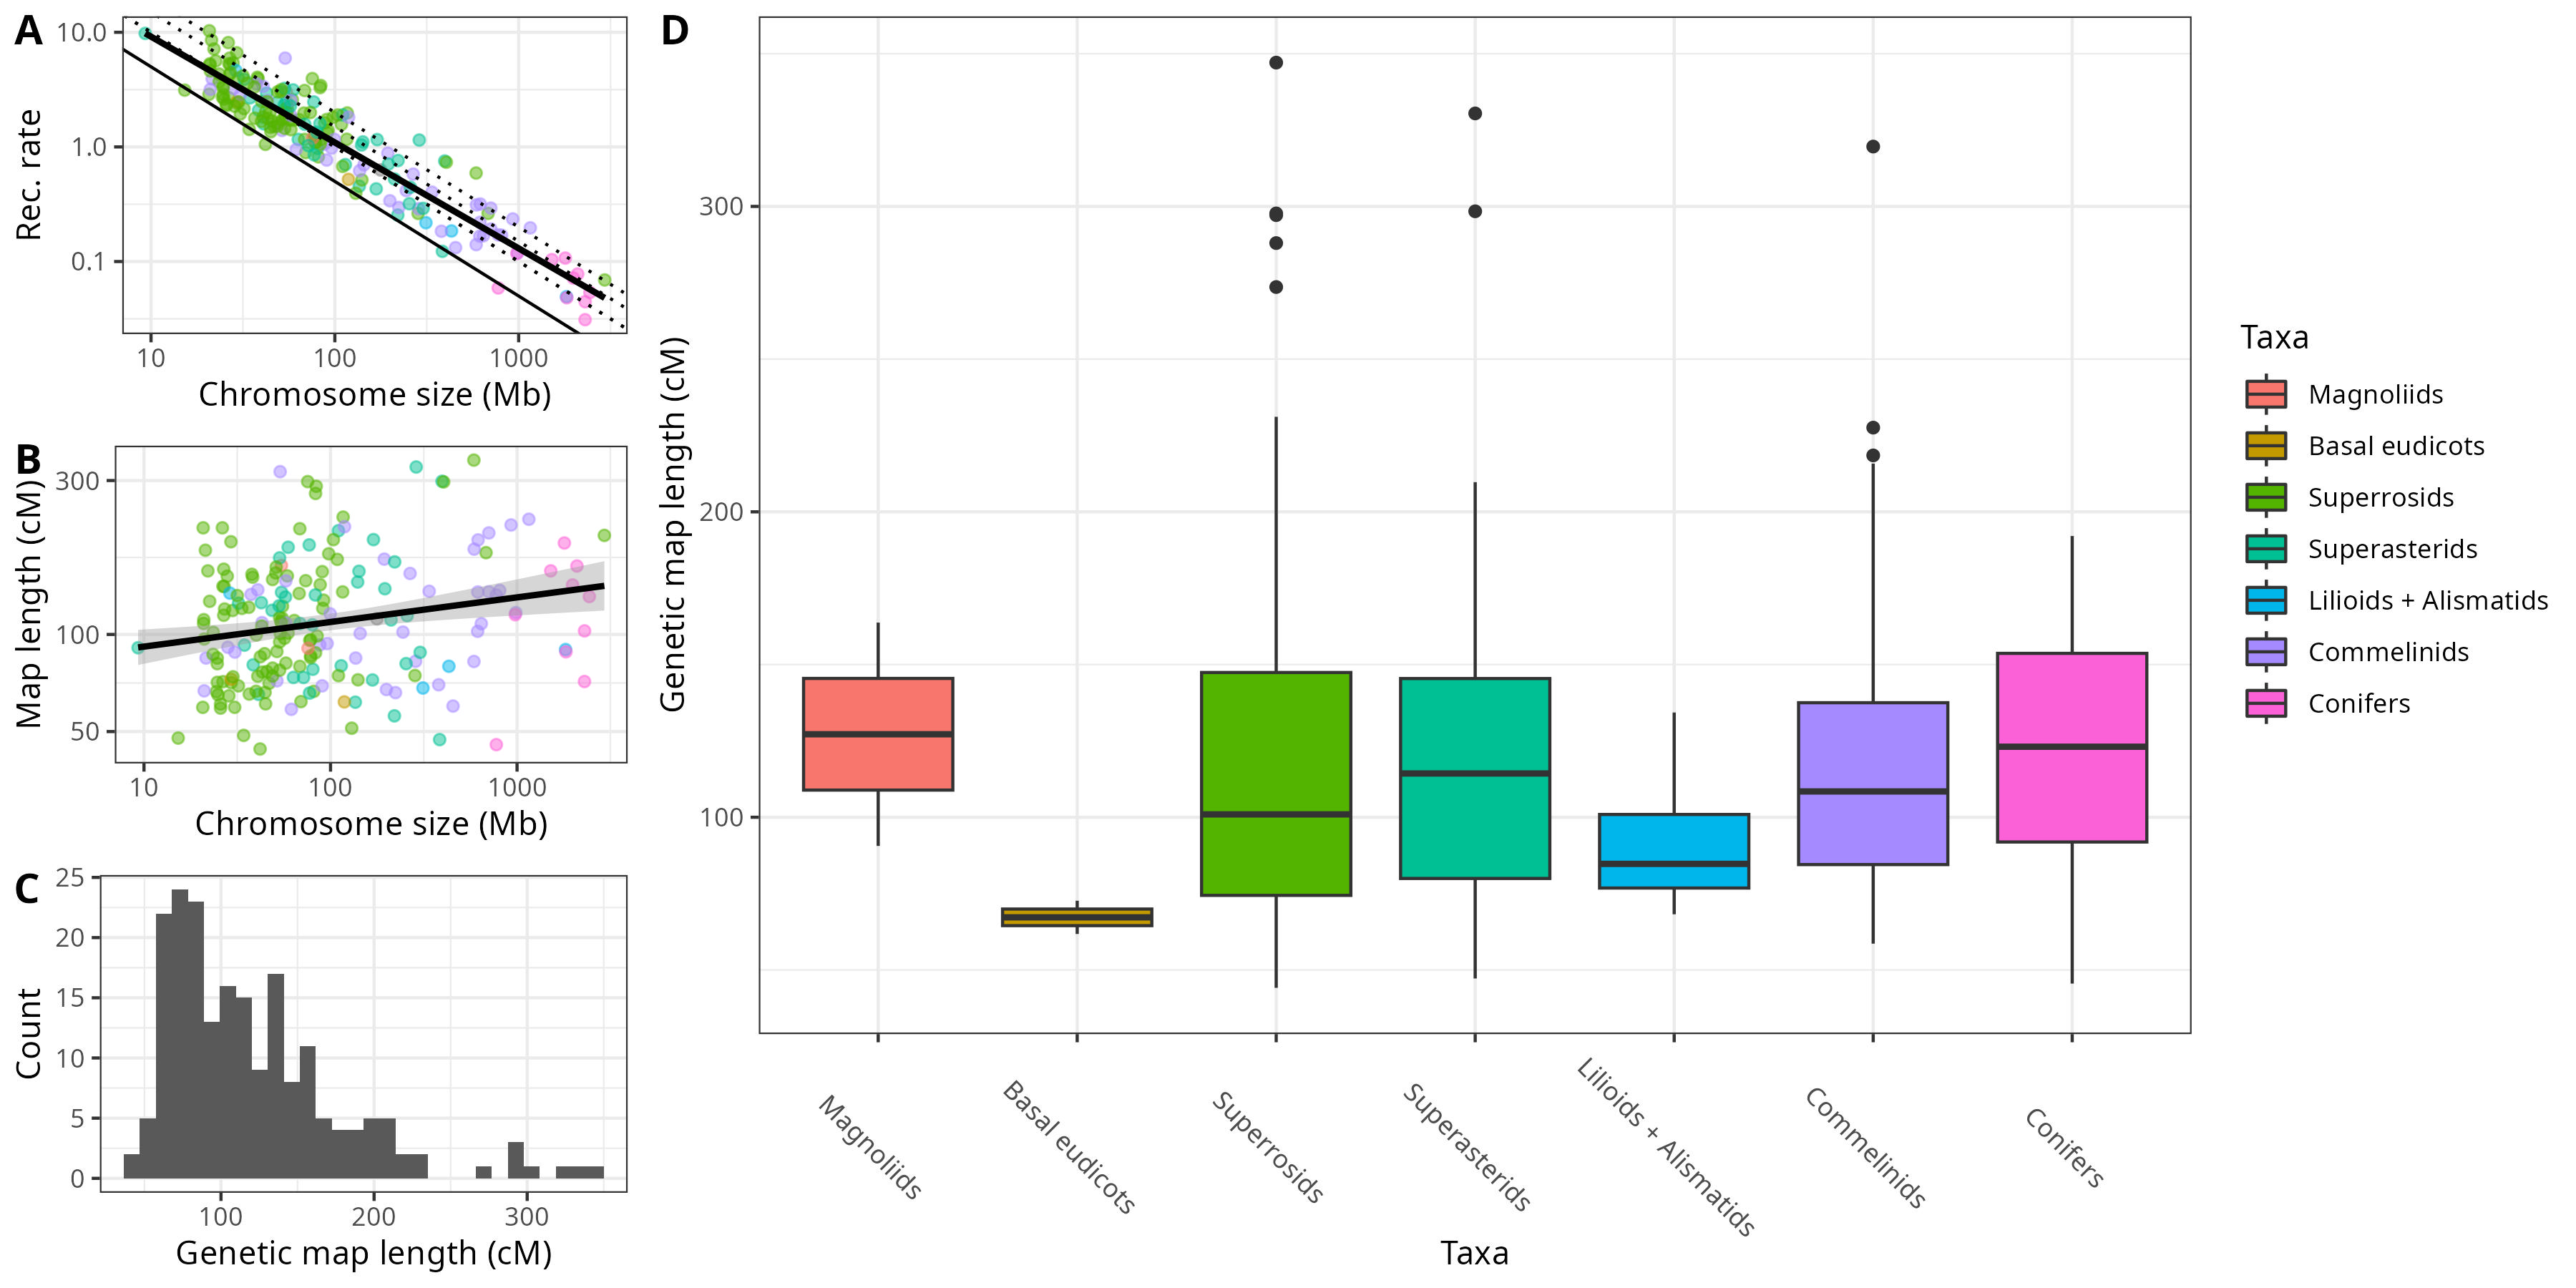
\includegraphics[width=0.9\textwidth]{figures/Fig1.jpeg}
  \centering
  \caption{Distribution of recombination rates and genetic map length  (n = 200 species). (A) Average chromosome size (Mb, log scale) is negatively correlated with recombination rates (cM/Mb, log scale). (B) Average genetic map length (cM) is weakly correlated to average chromosome size (Mb) (C) Density of chromosome genetic map length. (D) Boxplots of chromosome genetic map length per phylogenetic family. Compare with recombination rates (cM/Mb) in Figure 2 in Stapley et al. (\citeyear{stapleyVariationRecombinationFrequency2017}).
  }
  \label{figure:Fig1}
\end{figure}


\subsection*{Weak phylogenetic signal}


After controlling for the chromosome size effect, we also investigated how recombination rates evolved amongst the plant phylogeny. In order to test the significance and strength of the phylogenetic signal, we estimated two phylogenetic signal metrics (Blomberg’s K and Pagel’s lambda) and fitted three competing phylogenetic models (Brownian Motion, Ornstein-Uhlenbeck and Early-burst) to the continuous distribution of chromosome average genetic length and the residuals of the regression of recombination rates as a function of average chromosome size (Table \ref{table:table1}). Blomberg's K were not significantly different from zero while Pagel's Lambda was around 0.5, both indicating a weak phylogenetic signal. Based on the maximum Log-Likelihood criterion, the Ornstein-Uhlenbeck phylogenetic model was always preferred, suggesting that the recombination rate evolved under a constrained range.


\begin{table}[h!]
\centering{}
\caption{Phylogenetic signal for the two proxies of recombination rates. Blomberg’s K and Pagel’s Lambda (and their respective p-value) and the Log-Likelihood of the three phylogenetic models (Brownian Motion, Ornstein-Uhlenbeck and Early-burst, respectively). The best model according to the Log-Likelihood criterion is in bold.}
\begin{tabular}{llllllll}
Trait                      & K    & K p-value & $\lambda$ & $\lambda$ p-value & Log-lik BM & Log-lik OU & Log-lik EB \\ \hline
Genetic map length & 0.09 & 0.117                                         & 0.46   & 0.01     & -1155.09   & \textbf{-1091.53}                                             & -1155.09                                             \\
Residuals                  & 0.1  & 0.032                                         & 0.47   & 0.01     & -173.16    & \textbf{-110.77}                                              & -173.16                                             
\end{tabular}
\label{table:table1}
\end{table}




\subsection*{Joint effect of the mating system and longevity}


Based on ANOVAs and AIC/BIC criterion, we run a step forward model selection for Linear Regression and Phylogenetic Generalized Least Squares (Table \ref{table:tableS2}). For both average chromosome map length and the residuals, the two significant predictors were always the mating system first, then longevity based on ANOVA (p < 0.05) and AIC (lower AIC value). However these effects were weak (Figure \ref{figure:FigS3}, \ref{figure:FigS4}), as the null model was always preferred by the BIC criterion. The effect of other life history traits was weak or null. The more complex models including both mating system and longevity were significantly better than the two models with a single predictor, except for the Linear Model with the average chromosome map length as response variable (df = 2, F = 1.9095, p = 0.151). The effect was stronger when the phylogeny was accounted for (p = 0.035 for ‘lm’ vs. p = 0.008 for ‘pgls’). Overall, we observed a joint effect of the mating system and longevity on proxies of recombination rates (Figure \ref{figure:Fig2}, \ref{figure:FigS5}).



\begin{figure}[h!]
  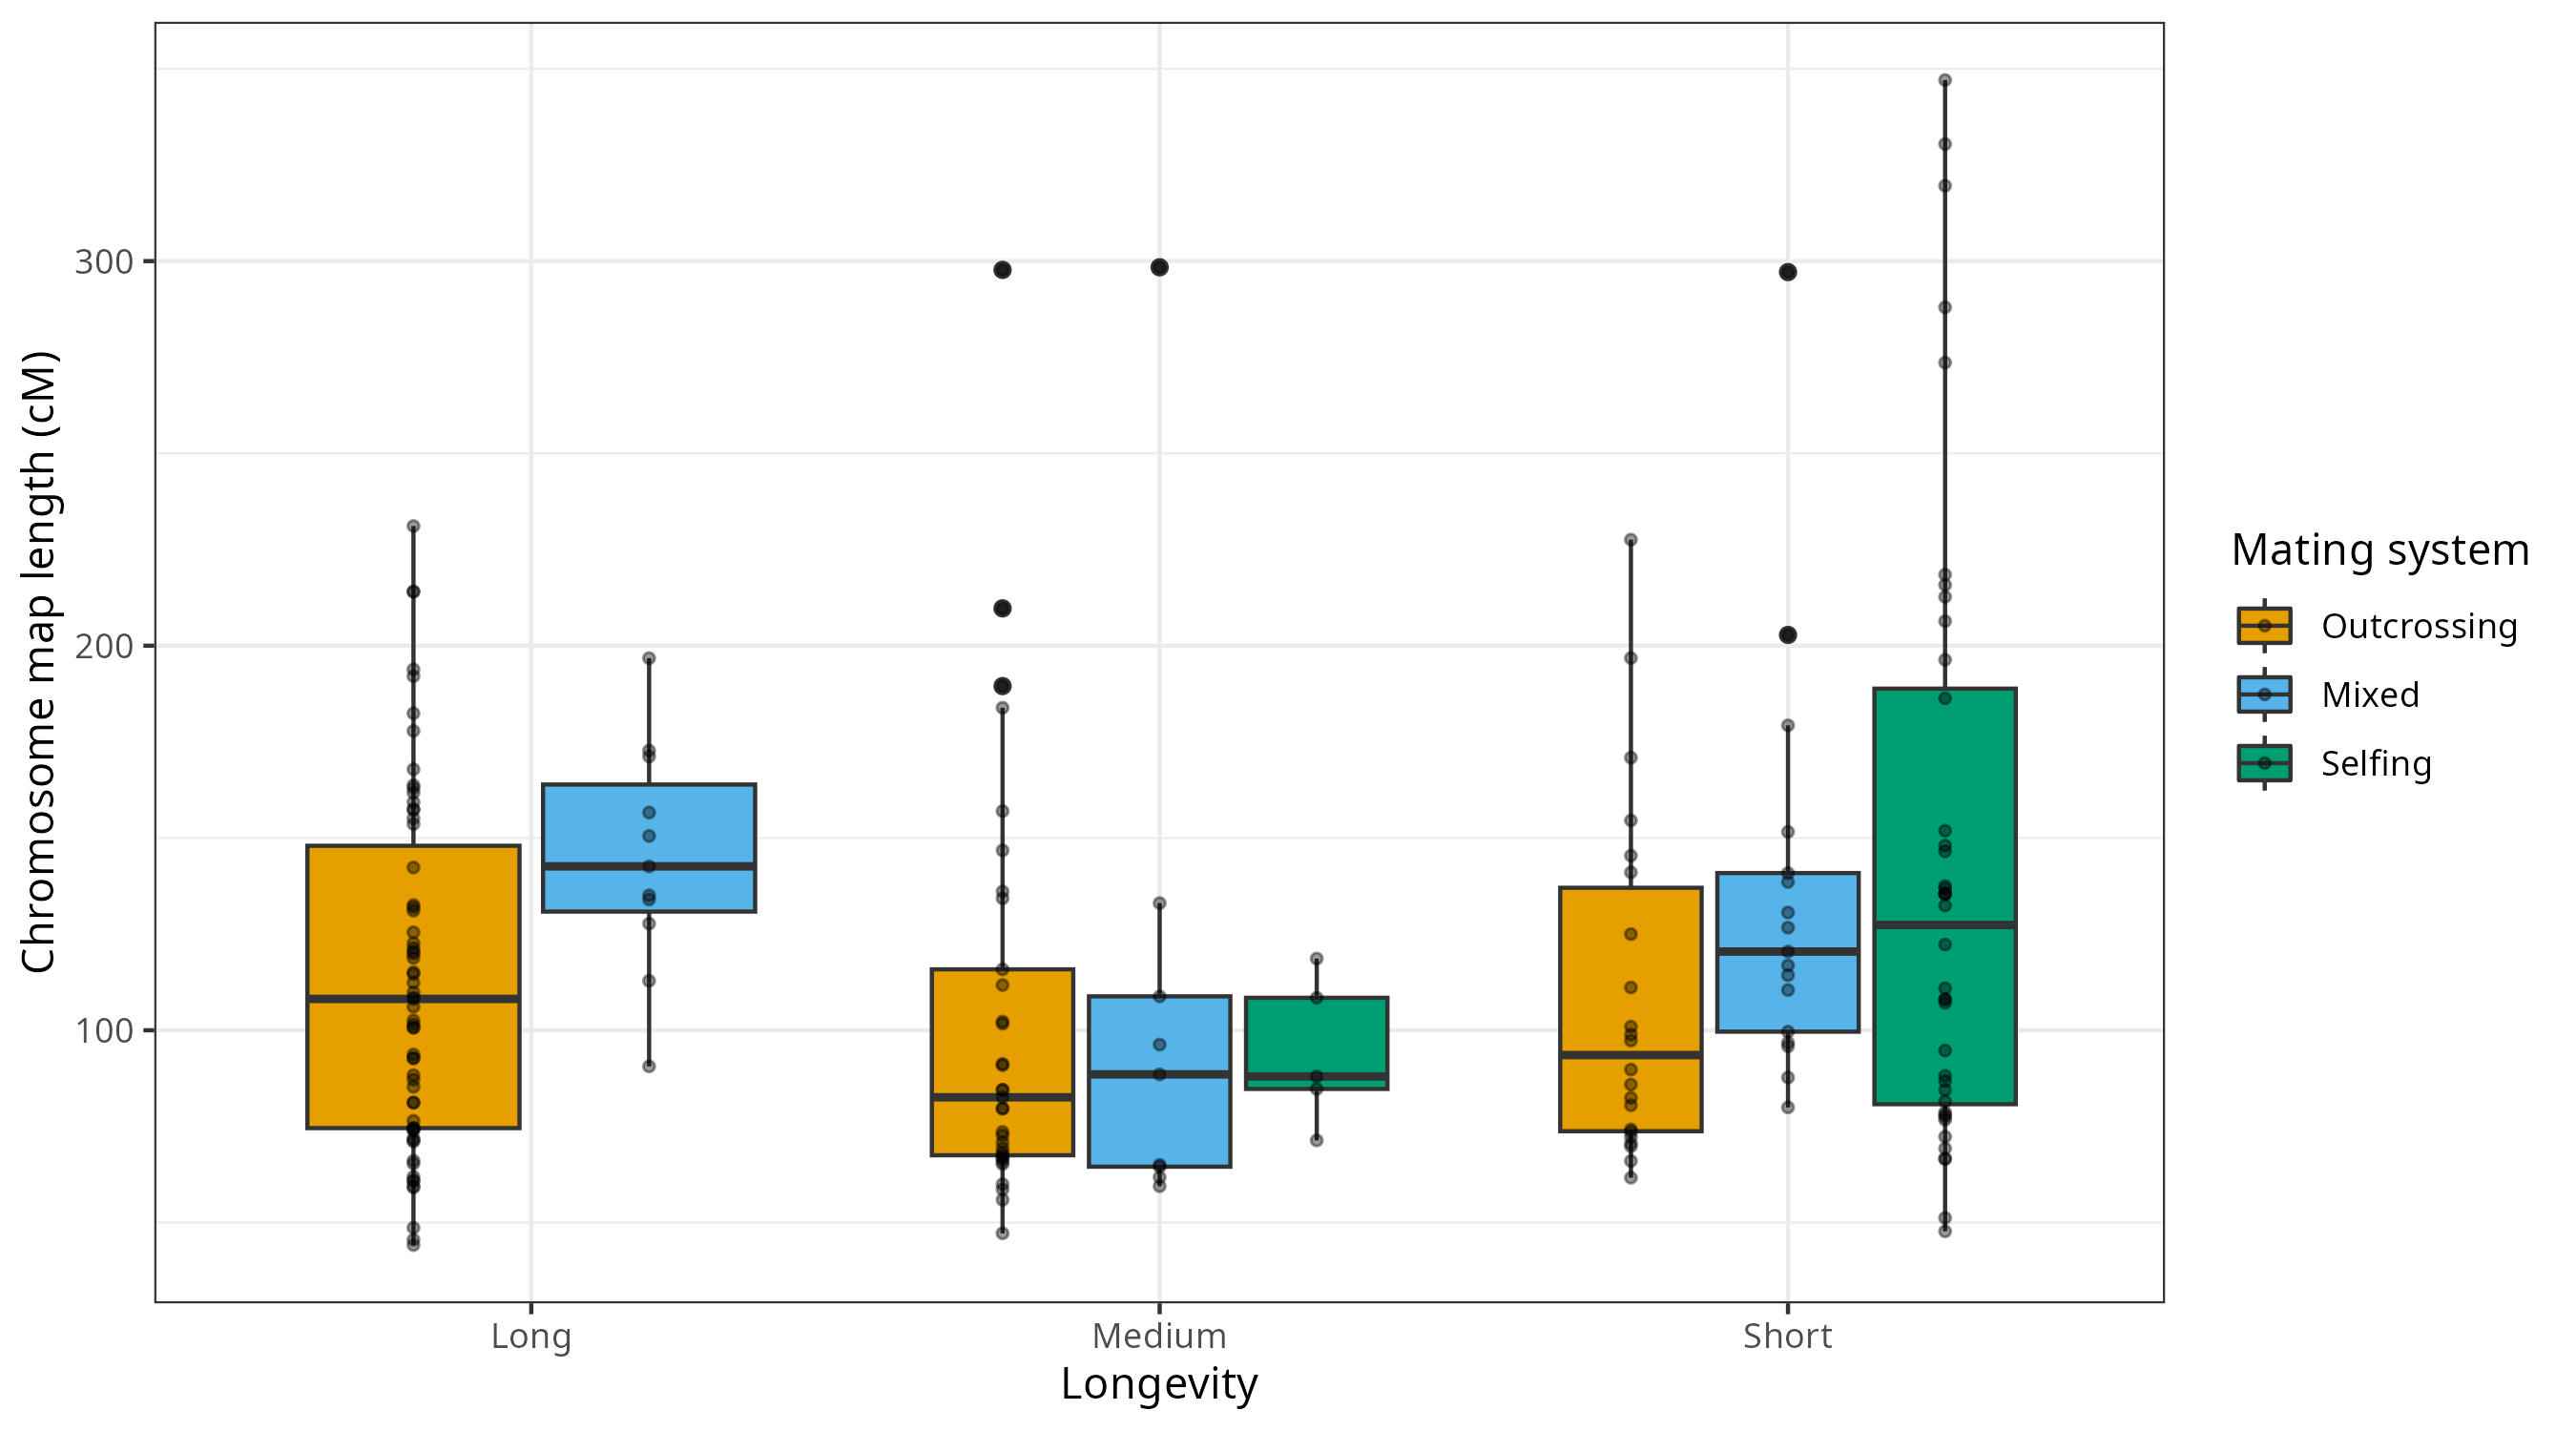
\includegraphics[width=0.9\textwidth]{figures/Fig2.jpeg}
  \centering
  \caption{Recombination rates depend on the mating system and longevity. (A) The combined effect of the mating system and longevity on the average chromosome genetic map length. Each point is a species (n = 200 species).
  }
  \label{figure:Fig2}
\end{figure}


\begin{table}[h!]
\centering{}
\caption{Model fit and parameter estimates of the best model (PGLS residuals ~ mating system + longevity, $\lambda$ = 0.480, F-statistic = 4.069, df = 195, p = 0.0034, Adjusted R-squared = 0.0581). Significance codes: 0 ‘***’ 0.001 ‘**’ 0.01 ‘*’ 0.05 ‘.’ 0.1 ‘ ’ 1.}
\begin{tabular}{llllllll}
Response                       & Df                 & p                       & Parameter        & Estimate & Std. Error & t       & p      \\ \hline
\multirow{3}{*}{Mating system} & \multirow{3}{*}{2} & \multirow{3}{*}{0.0078 **} & (Intercept)      & -0.0789  & 0.2145     & -0.368  & 0.7133 \\ \cline{4-8} 
                               &                    &                         & Mixed-mating     & 0.1805   & 0.0824     & 2.1898  & 0.0297 * \\
                               &                    &                         & Selfing          & 0.1857   & 0.0891     & 2.0839  & 0.0385 * \\ \cline{4-8} 
\multirow{2}{*}{Longevity}     & \multirow{2}{*}{2} & \multirow{2}{*}{0.0443 *} & Medium longevity & -0.2201  & 0.0941     & -2.3395 & 0.0203 * \\
                               &                    &                         & Short longevity  & -0.0741  & 0.0994     & -0.7461 & 0.4565
\end{tabular}
\label{table:table2}
\end{table}


As a final model we selected the Phylogenetic Generalized Least Squares with the residuals as a response variable ($\lambda$ = 0.480, F-statistic = 4.069, df = 195, p = 0.003433, Adjusted R-squared = 0.0581, Table \ref{table:table2}) where selfing and mixed mating species had significantly higher recombination than outcrossing species whereas medium-lived species had significantly lower recombination (Table \ref{table:table2}). Both the mating system and longevity were significant in the ANOVA (df = 2, Sum of Squares = 0.0076, Mean Squares = 0.0038, F = 4.9710, p = 0.0078, and df = 2, Sum of Squares = 0.0048, Mean Squares = 0.0024, F = 3.1666, p = 0.0443, respectively). The validity of the model was successfully assessed with diagnostic plots. The model with the average genetic map length yielded similar results.


We observed the same results when we plotted the joint effect of the mating system and longevity on recombination rates (Figure \ref{figure:Fig2}, \ref{figure:FigS5}). Outcrossing species had on average lower recombination rates for the three longevity categories though the difference was less clear in medium-lived species. On average, selfing and mixed mating system species had higher recombination rates. There was no selfing species in long-lived species. Medium-lived species had lower recombination rates on average, with globally a maximum of two COs per chromosome (i.e. 100 cM) while long and short-lived generally exceeded two COs.


\subsection*{Selection for higher recombination varies among phylogenetic families}


We investigated if there could be a family-specific effect of the mating system or longevity. Our phylogenetic sampling was sparse across the plant phylogeny but we managed to subset three independent families with at least ten species each and two species for each mating system. The family-specific selfing effect was not clear among the three families (Figure \ref{figure:Fig3}A). The increased recombination rate in selfing species was clear in Poaceae but weak or even reversed in Brassicaceae and Fabaceae. We observed only a few mixed-mating species. For Fabaceae and Poaceae we observed a clear short-lived effect with increased recombination rates (Figure \ref{figure:Fig3}B). We did not have enough medium-lived species to conclude for Brassicaceae. We did not have enough samples to investigate the joint effect or to perform a proper statistical analysis.



\begin{figure}[h!]
  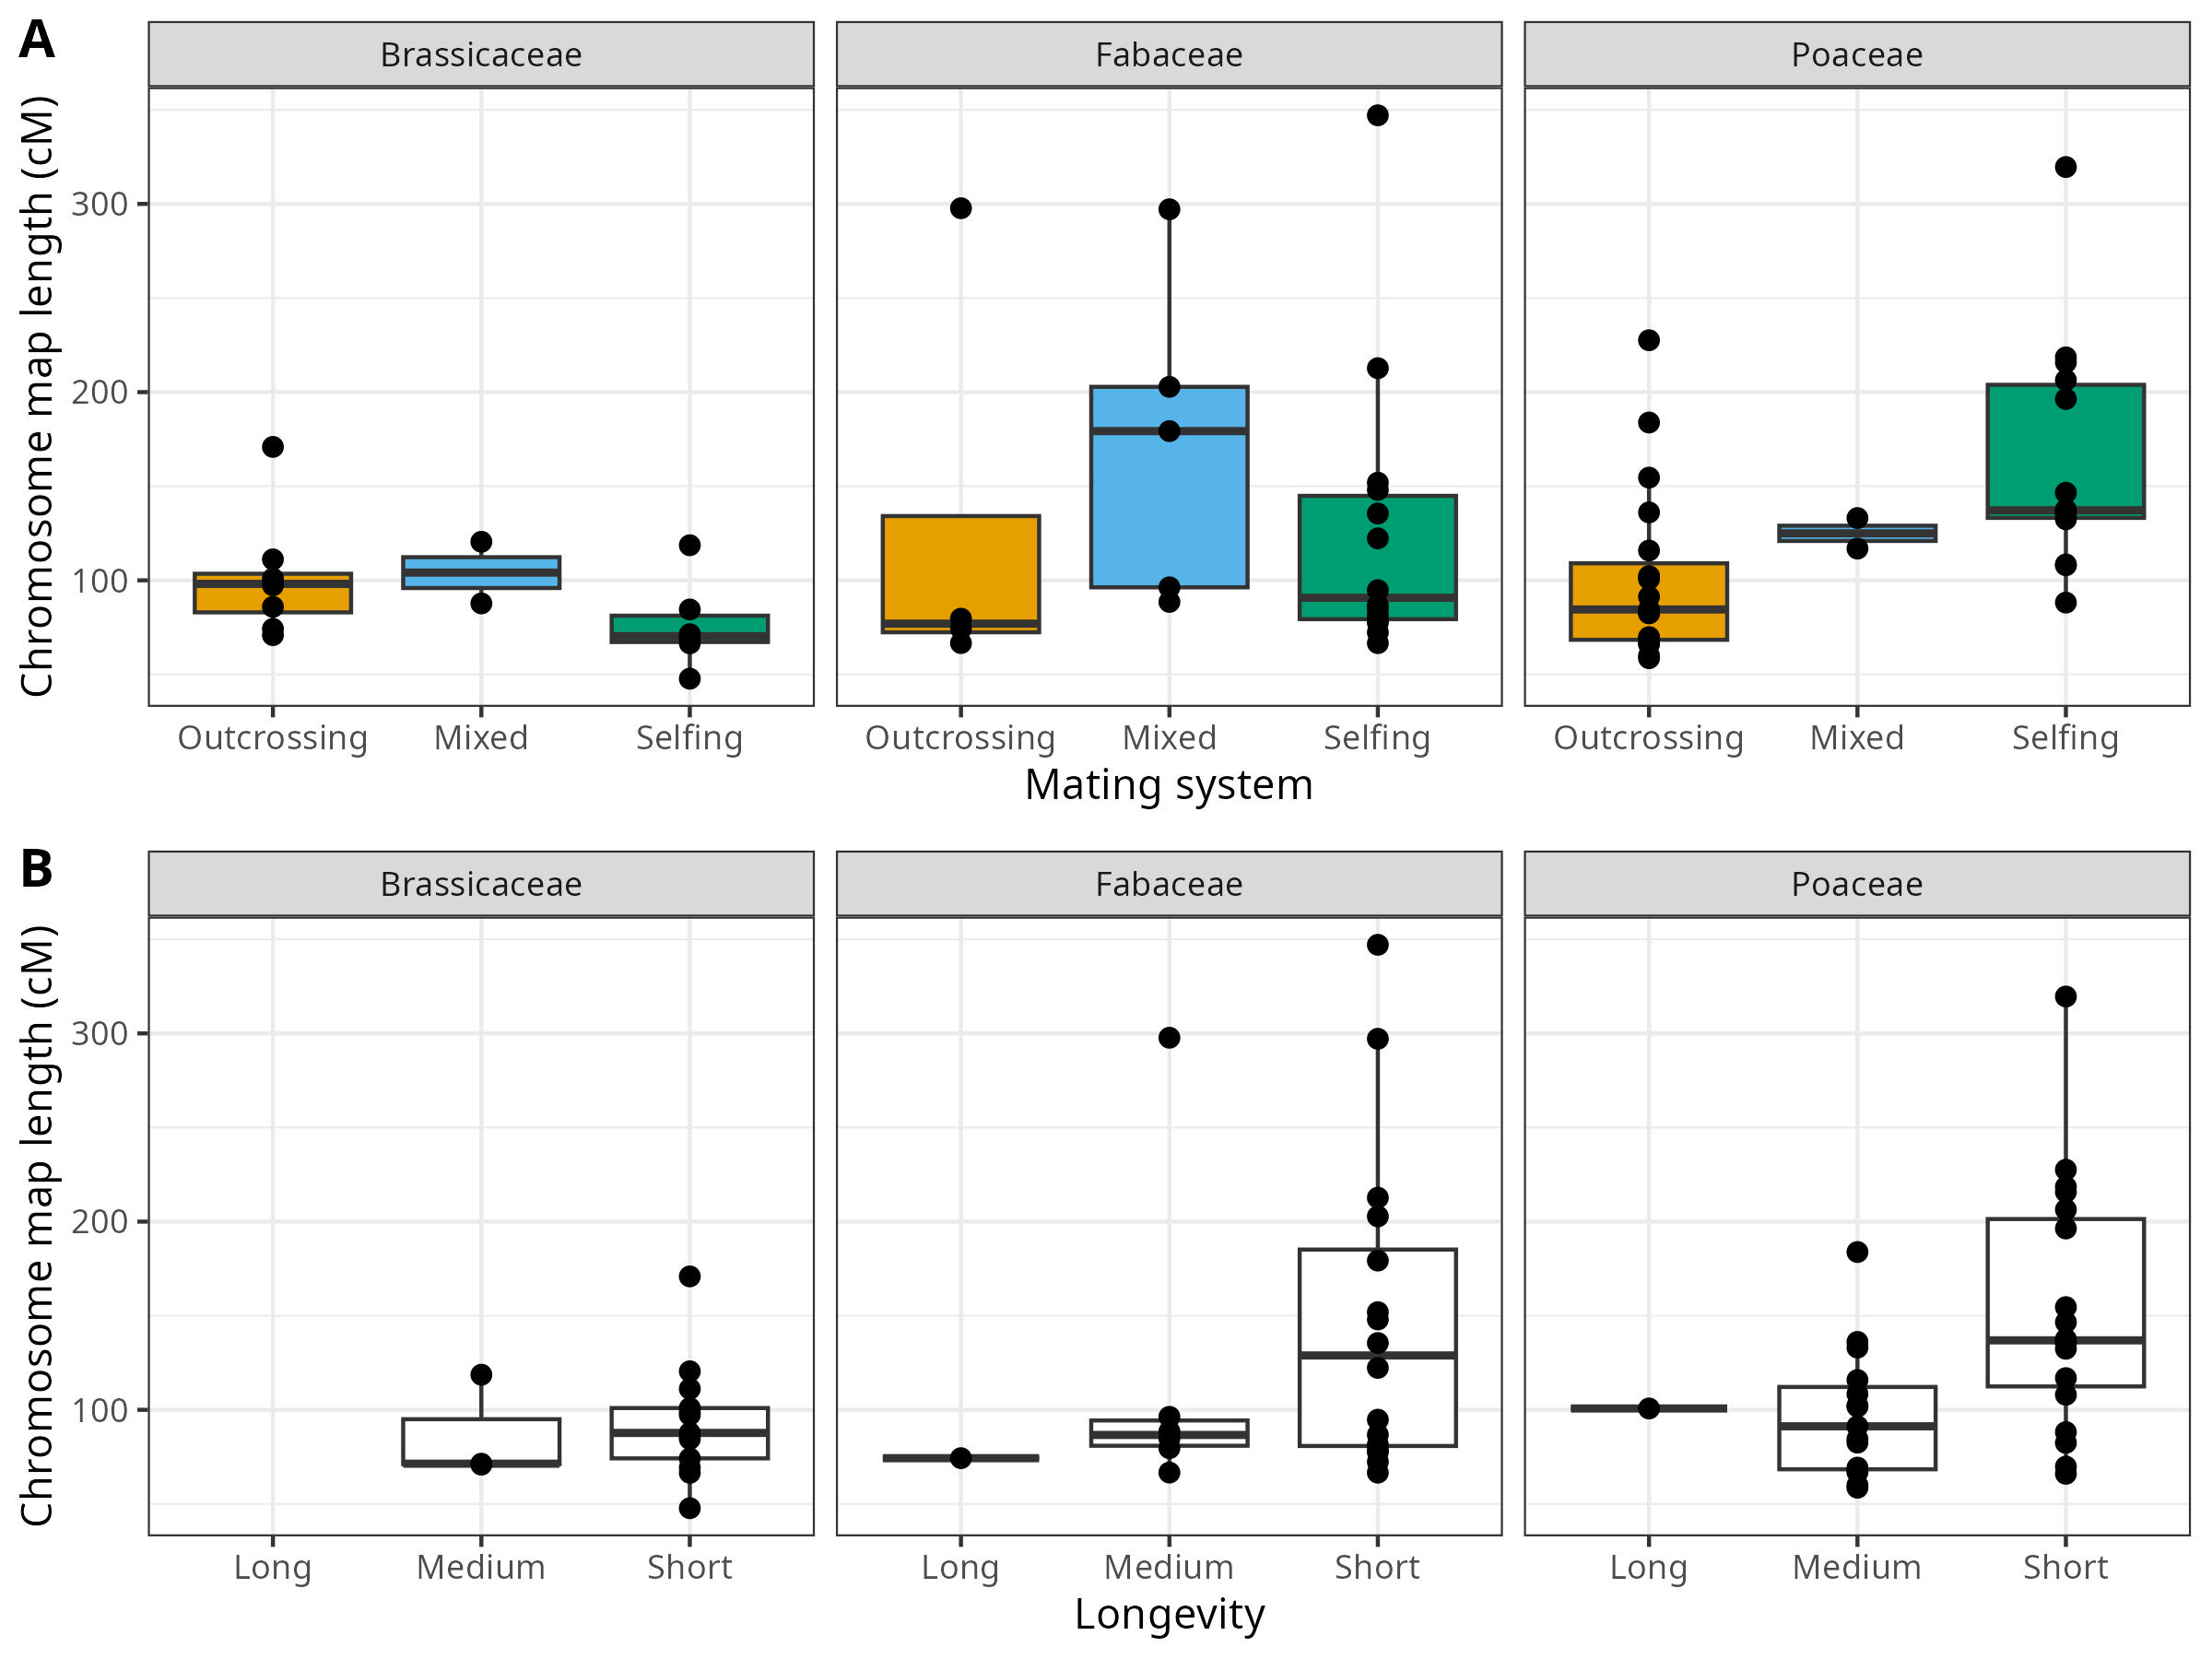
\includegraphics[width=0.9\textwidth]{figures/Fig3.jpeg}
  \centering
  \caption{Chromosome genetic map length as a function of the mating system (same colors as in Figure \ref{figure:Fig2}) or longevity in three different phylogenetic families (n = 91 species). Each point is a species.
  }
  \label{figure:Fig3}
\end{figure}



\subsection*{Selection towards extra crossovers in selfing and mixed mating species}


We analyzed the dataset slightly differently by considering that there is one mandatory CO per chromosome and then the additional number of CO can increase or not with chromosome size, depending on the strength of CO interference. If CO interference is limited, larger chromosomes should have on average a higher number of COs. On the contrary, if interference is the limiting factor, evolution towards more COs on larger chromosomes should be prevented. We tested this idea by analyzing separately for each mating system the slope of the average chromosome genetic map length as a function of chromosome physical size (Figure \ref{figure:Fig4}). Species with larger chromosomes seemed to have more COs per chromosome in selfing and mixed-mating species but not in outcrossing species. The intercept was similar among the three mating systems (Figure \ref{figure:Fig4}). We tested the significance of this effect with a PGLS model with an interaction term between the chromosome size and the mating system. We also used the number of chromosomes as a covariate, since the Genome Wide Recombination Rate can be increased by increasing the total number of chromosomes (chromosome genetic map length ~ chromosome size*mating system + number of chromosomes, $\lambda$ = 0.468, F-statistic = 3.732, df = 193, p = 0.0016, Adjusted R-squared = 0.0761). There was a trend for the interaction between chromosome size and the mating system (p = 0.056), as well as a trend for the number of chromosomes (p = 0.071; see Table \ref{table:tableS3} for model fit and parameters). While there was a slight trend for the chromosomal genetic map length to increase with chromosome size in selfing species (interaction chromosome size:selfing, coefficient = 0.069, std. error = 0.0359, t = 1.9229, p = 0.056), the number of chromosomes had a negative effect on the chromosomal genetic map length (coefficient = -0.946, std. error = 0.5213, t = -1.8147, p = 0.0711).




\begin{figure}[h!]
  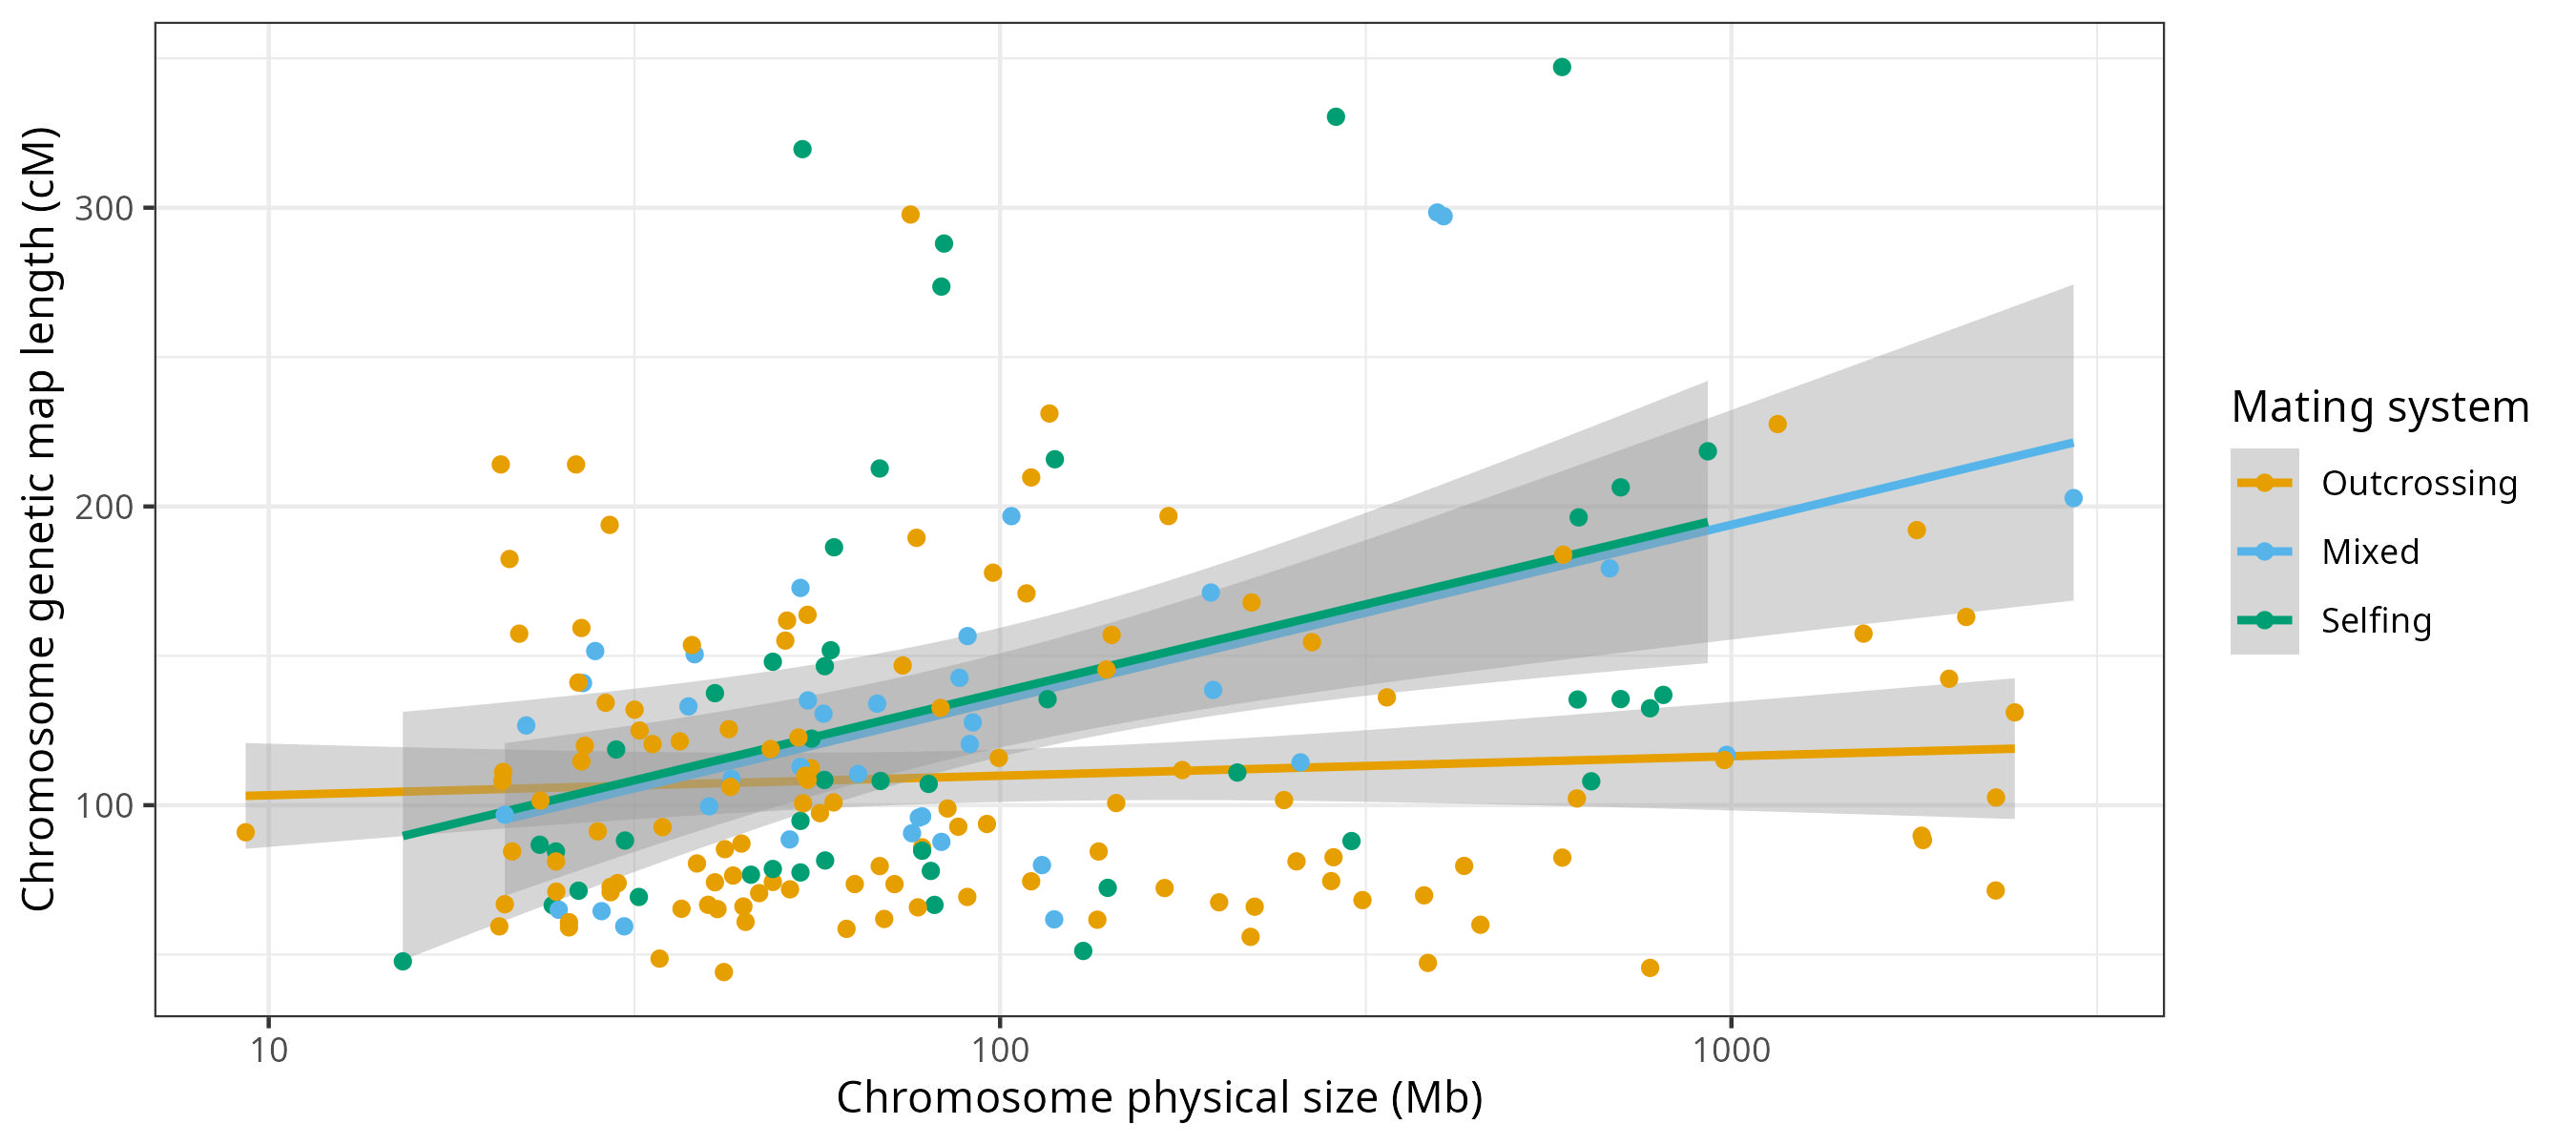
\includegraphics[width=0.9\textwidth]{figures/Fig4.jpeg}
  \centering
  \caption{Selection towards higher CO rates in larger chromosomes for selfing and mixed-mating species (n = 118, 37 and 45 for outcrossing, mixed-mating and selfing species, respectively). The linear regression line and its 95\% confidence interval for each mating system were estimated with the ggplot2 'geom\_smooth' function (\cite{wickhamGgplot2ElegantGraphics2016}).}
  \label{figure:Fig4}
\end{figure}



\subsection*{The effect is robust to map quality}


In order to control if the mating system and longevity effect were robust to differences in map quality among species, we tested the influence of marker density and number of progenies on the significance of the results. We added either marker density or number of progenies to the Phylogenetic Generalized Least Squares model with the residuals as a response variable. Marker density had a significant positive effect on recombination rates (p = 0.028035, see parameter estimates in Table \ref{table:tableS4}) but it did not change the significance of selfing and medium-lived species (p = 0.0469 and 0.0318, respectively) while mixed-mating species remained as a trend (p = 0.0681). Progeny number was not significant at all (p = 0.5988).


\section*{Discussion}

In order to test for an effect of the mating system on the evolution of recombination rates, we compared genetic maps in 200 plant species differing by their mating system and other life-history traits. We found a joint positive effect of the mating system and longevity on recombination rates with variation across phylogenetic families. We also found that mixed-mating and selfing species had a significantly higher number of crossovers in larger chromosomes compared to outcrossing species. These results have implications for the evolution of recombination given the constraints imposed on the number of crossovers per chromosome.


\subsection*{Higher CO rates in selfing and mixed-mating species}


Among life history traits, the mating system has the main significant effect on recombination rates after controlling for the strong chromosome size effect. Indeed, chromosome size is a major determinant of recombination rates in Eukaryotes (\cite{brazierDiversityDeterminantsRecombination2022b,stapleyVariationRecombinationFrequency2017,haenelMetaanalysisChromosomescaleCrossover2018}) but our results show that the average chromosome genetic map length (i.e. the average number of COs) is only weakly proportional to chromosome size. The average number of COs per chromosome varies between one and four for most species, with some species exceeding six COs per chromosome (300 cM). Despite constraints on the number of COs per chromosome, as supported by the choice of the OU model (Table \ref{table:table1}), there is still possible variation upon which selection can act.


Selfing and mixed-mating species have higher recombination rates on average than outcrossing species, thus supporting the theoretical predictions of a positive effect of selfing on recombination(\cite{rozeSelfFertilizationEvolutionRecombination2005,stetsenkoEvolutionRecombinationSelffertilizing2022}). Under realistic parameter values, Stetsenko and Roze (\citeyear{stetsenkoEvolutionRecombinationSelffertilizing2022}) found that selfing increases selection for recombination to compensate for the decreased efficacy of recombination. However, they predict that selection for recombination vanishes for selfing rates approaching one as, in this case, homozygosity is too high for recombination to have an effect. This results in a non-monotonic increase in recombination with selfing, with the selfing rate maximizing selection for recombination depending on parameter values, but typically being quite high. Our data are not precise enough to directly assess the nature of the relationship between selfing rate and recombination rate. However, we observed the main difference between outcrossing and mixed-mating + selfing, with no significant difference between mixed mating and selfing, which is in agreement with the non-linear relationship predicted by theory assuming particular forms of epistasis between deleterious mutations.


Our study also matches well with previous empirical results. Cytological measures of the number of chiasmata per bivalent per meiosis in several plant genera tend to confirm this overall increase of recombination with selfing (reviewed in \cite{rozeSelfFertilizationEvolutionRecombination2005} and \cite{ross-ibarraGenomeSizeRecombination2007a}). This positive correlation was found to be significant across all species as well as within genera (\cite{rozeSelfFertilizationEvolutionRecombination2005}). However, chiasma frequency only represents an indirect measure of the genome-wide recombination rate and is only available in a dozen genera. Similar results were found from genetic maps, pointing at higher recombination rates in the highly selfing \textit{Arabidopsis thaliana} compared to its outcrossing relative \textit{Arabidopsis lyrata} (\cite{hanssonComparativeGeneMapping2006a,kawabeComparativeGeneMapping2006,kuittinenComparingLinkageMaps2004}), but it was only in a single pair of species.


We observed a significant joint effect of the mating system and longevity. Recombination rates are similar at the extreme life-spans, in short and long-lived species (annual and woody perennial, respectively), while medium-lived species (perennial non-woody species such as herbs and vines) experience lower recombination rates on average. Taking longevity into account reveals a stronger effect of the mating system in short- and long-lived species than in medium-lived species (note that long-lived selfing species are exceedingly rare and absent from our dataset). In mammals, Burt and Bell (\cite{burtMammalianChiasmaFrequencies1987}) proposed that a long life-span should select more recombination but the mechanism remains unclear. In plants, a meta-analysis on chiasma frequencies found lower recombination in perennials than in annual species, but they did not distinguish medium- and long-lived perennials and did not control for the mating system as we did (\cite{koellaEcologicalCorrelatesChiasma1993}).


\subsection*{Indirect evidence of reduced CO interference to increase the CO number}


The CO number per chromosome per meiosis is strongly constrained by CO assurance and interference (\cite{wangMeioticCrossoverPatterns2015}). While CO assurance guarantees at least one CO, the maximum number of COs is strongly limited by CO interference, up to a maximum of four COs in most species (\cite{brazierDiversityDeterminantsRecombination2022b,stapleyVariationRecombinationFrequency2017}). This limited evolvability probably explains why the mating system and longevity have a marginal effect that is significant only after controlling for the strong chromosome size effect. The proxies of recombination rates have a weak phylogenetic signal and the Ornstein-Uhlenbeck model of evolution is always preferred, suggesting stabilizing selection on the number of COs.


However indirect selection on the strength of CO interference might be a possible mechanism to allow evolution towards a higher CO number, especially in non-random mating populations. The strength of CO interference itself varies dramatically among species (\cite{ottoCrossoverInterferenceShedding2019}) and CO interference is thought to evolve in finite populations as a way to reduce selective interference among loci (\cite{barton2005evolution,keightley2006interference,roze2006hill}). Indeed we observe a higher number of COs per chromosome in mixed-mating and selfing species, particularly in larger chromosomes, while this trend is not observed in outcrossing species. This suggests that the higher number of COs in mixed-mating and selfing species may evolve through relaxed CO interference allowing more COs to occur on the same chromosome. On the contrary, CO interference may have remained strong in outcrossing species, limiting the CO number to its minimum independently of chromosome size.


One interesting question is whether one or two extra COs are sufficient to efficiently compensate for the reduced efficiency of selection due to selfing. Considering that most of the genetic shuffling is done via the independent assortment of chromosomes (inter-chromosomal shuffling), a more efficient way to increase the recombination rate would be increasing the chromosome number to produce more COs on the whole (\cite{vellerRigorousMeasureGenomewide2019}). Selection for increased number of COs per chromosome, increased by the effect of selfing, should thus be stronger in species with a small number of chromosomes. The number of COs per chromosome can evolve more rapidly than the number of chromosomes, possibly on the same timescale as selfing rates (\cite{hendersonEvolutionPlasticityGenomeWide2021,whiteheadPlantMatingSystems2018}). It is thus more likely that the number of chromosomes constrains the evolution of CO number rather than being the direct target of selection for increased genetic shuffling. We found that at a chromosome level, the number of chromosomes was negatively associated with the chromosome genetic map length, though not significantly. At a genome wide level, Stapley et al. (\citeyear{stapleyVariationRecombinationFrequency2017}) found a weak positive effect of chromosome number on the genome wide recombination rate (cM/Mb) in plants, but not in animals and fungi.


\subsection*{Strength and limitations of our dataset}


The effect of the mating system and longevity is moderate, most likely because it is biologically much weaker than the dominant chromosome size effect. We were able to detect it by leveraging a large curated dataset from Stapley et al. (\citeyear{stapleyVariationRecombinationFrequency2017}) plus 24 new species with a sampling across seed plants (angiosperms and gymnosperms). We also found that the results were robust to differences in map quality (approximated by marker density and number of progeny).


However, our dataset remains limited to detect complex effects. The interaction between chromosome size and the mating system is only a trend. We did not detect significant effects for other life-history traits, despite strong expectations for some of them (e.g. cultivation status). There is multiple evidence of an effect of domestication on recombination rates in plants (\cite{ross-ibarraGenomeSizeRecombination2007a,dreissigVariationRecombinationRate2019,fuentesDomesticationShapesRecombination2021,schreiberRecombinationLandscapeDivergence2022}). However, we were not able to distinguish cultivated and domesticated species in our dataset and many species can be either strongly domesticated or wild relative populations. For such traits, a pairwise sampling of closely related species/populations with contrasted life history traits (wild vs. domesticated) should be more powerful than our large unstructured sampling. In particular, comparing species with the same number of chromosomes and similar genome size would avoid the strong confounding effect of chromosome size. It is likely that such an approach would also strengthen the detection of the effect of the mating system.


It is difficult to empirically test theories on the evolution of recombination and comparative analyses are a valuable approach as a first step to identify relevant factors. Despite the limitations discussed above, our results point to the mating system as an important factor potentially shaping the evolution of recombination. Further detailed studies of recombination patterns in species with contrasting selfing rates is a promising approach to better understand the forces acting on the evolution of recombination and, in turn, the evolution of selfing rates.




\section*{Acknowledgments}



We thank Laetitia Carrive for discussions about plant phylogeny.



\section*{Funding}

Agence Nationale de la Recherche, Grant ANR-19-CE12472 0019 / HotRec. 


\section*{Author contributions}

T.B. and S.G. gathered the data and did the analyses. R.S. and D.R. discussed the results. All authors equally wrote the draft and revised the manuscript.


\section*{Competing interests}

The authors declare no conflicts of interest.


\section*{Data availability} 

All scripts and data necessary to reproduce this study are available at the OSF repository \textbf{https://osf.io/XXX}.


\printbibliography


%%%%%%%%%%%%%%%%%%%%%%%%%%%%%%%%%%%%%%%%%%%%%%%%%%%%%%%%%%%%
%%% SUPPLEMENTARIES
%%%%%%%%%%%%%%%%%%%%%%%%%%%%%%%%%%%%%%%%%%%%%%%%%%%%%%%%%%%%


\section*{Supplementary figures}

\renewcommand{\thefigure}{S\arabic{figure}}

\setcounter{figure}{0}


\begin{figure}[h!]
  \includegraphics[width=0.9\textwidth]{figures/FigS1.jpeg}
  \centering
  \caption{Phylogeny of the complete dataset based on the ultra-metric tree from Smith and Brown (\citeyear{smithConstructingBroadlyInclusive2018}).
  }
  \label{figure:FigS1}
\end{figure}



\begin{figure}[h!]
  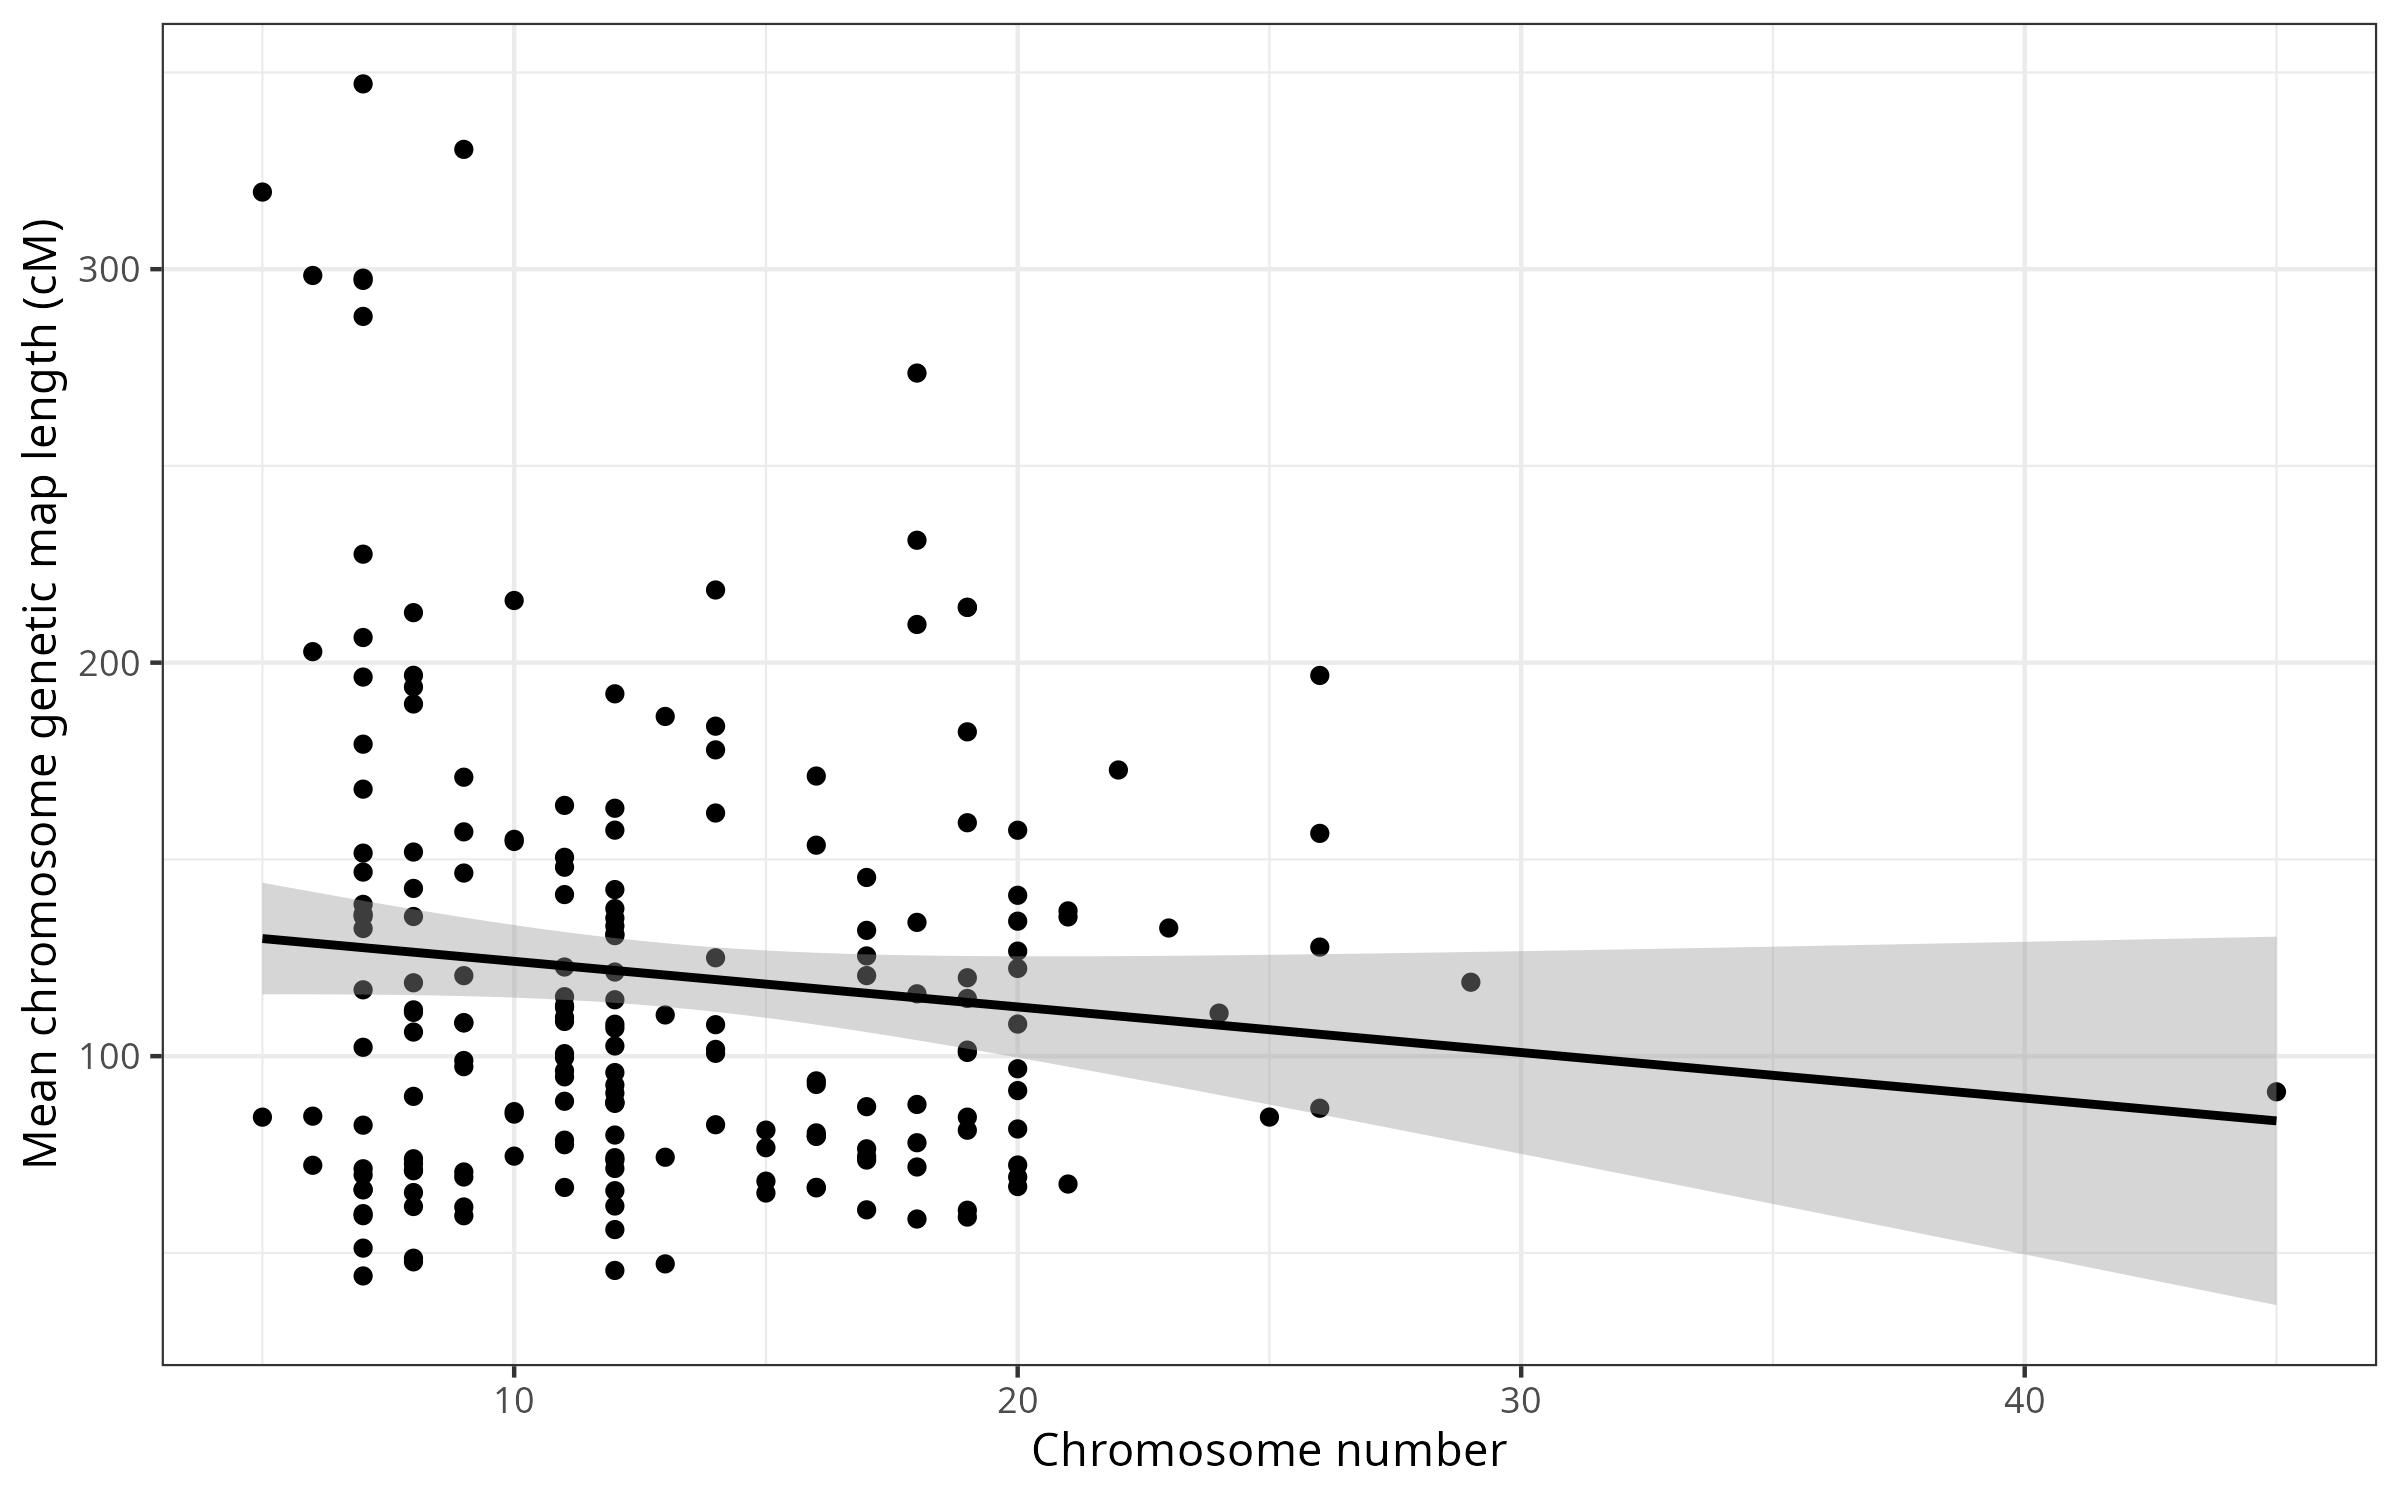
\includegraphics[width=0.9\textwidth]{figures/FigS2.jpeg}
  \centering
  \caption{Average chromosome map length is not correlated with the haploid chromosome number (Spearman’s $\rho$ = -0.08, p = 0.27).
  }
  \label{figure:FigS2}
\end{figure}


\begin{figure}[h!]
  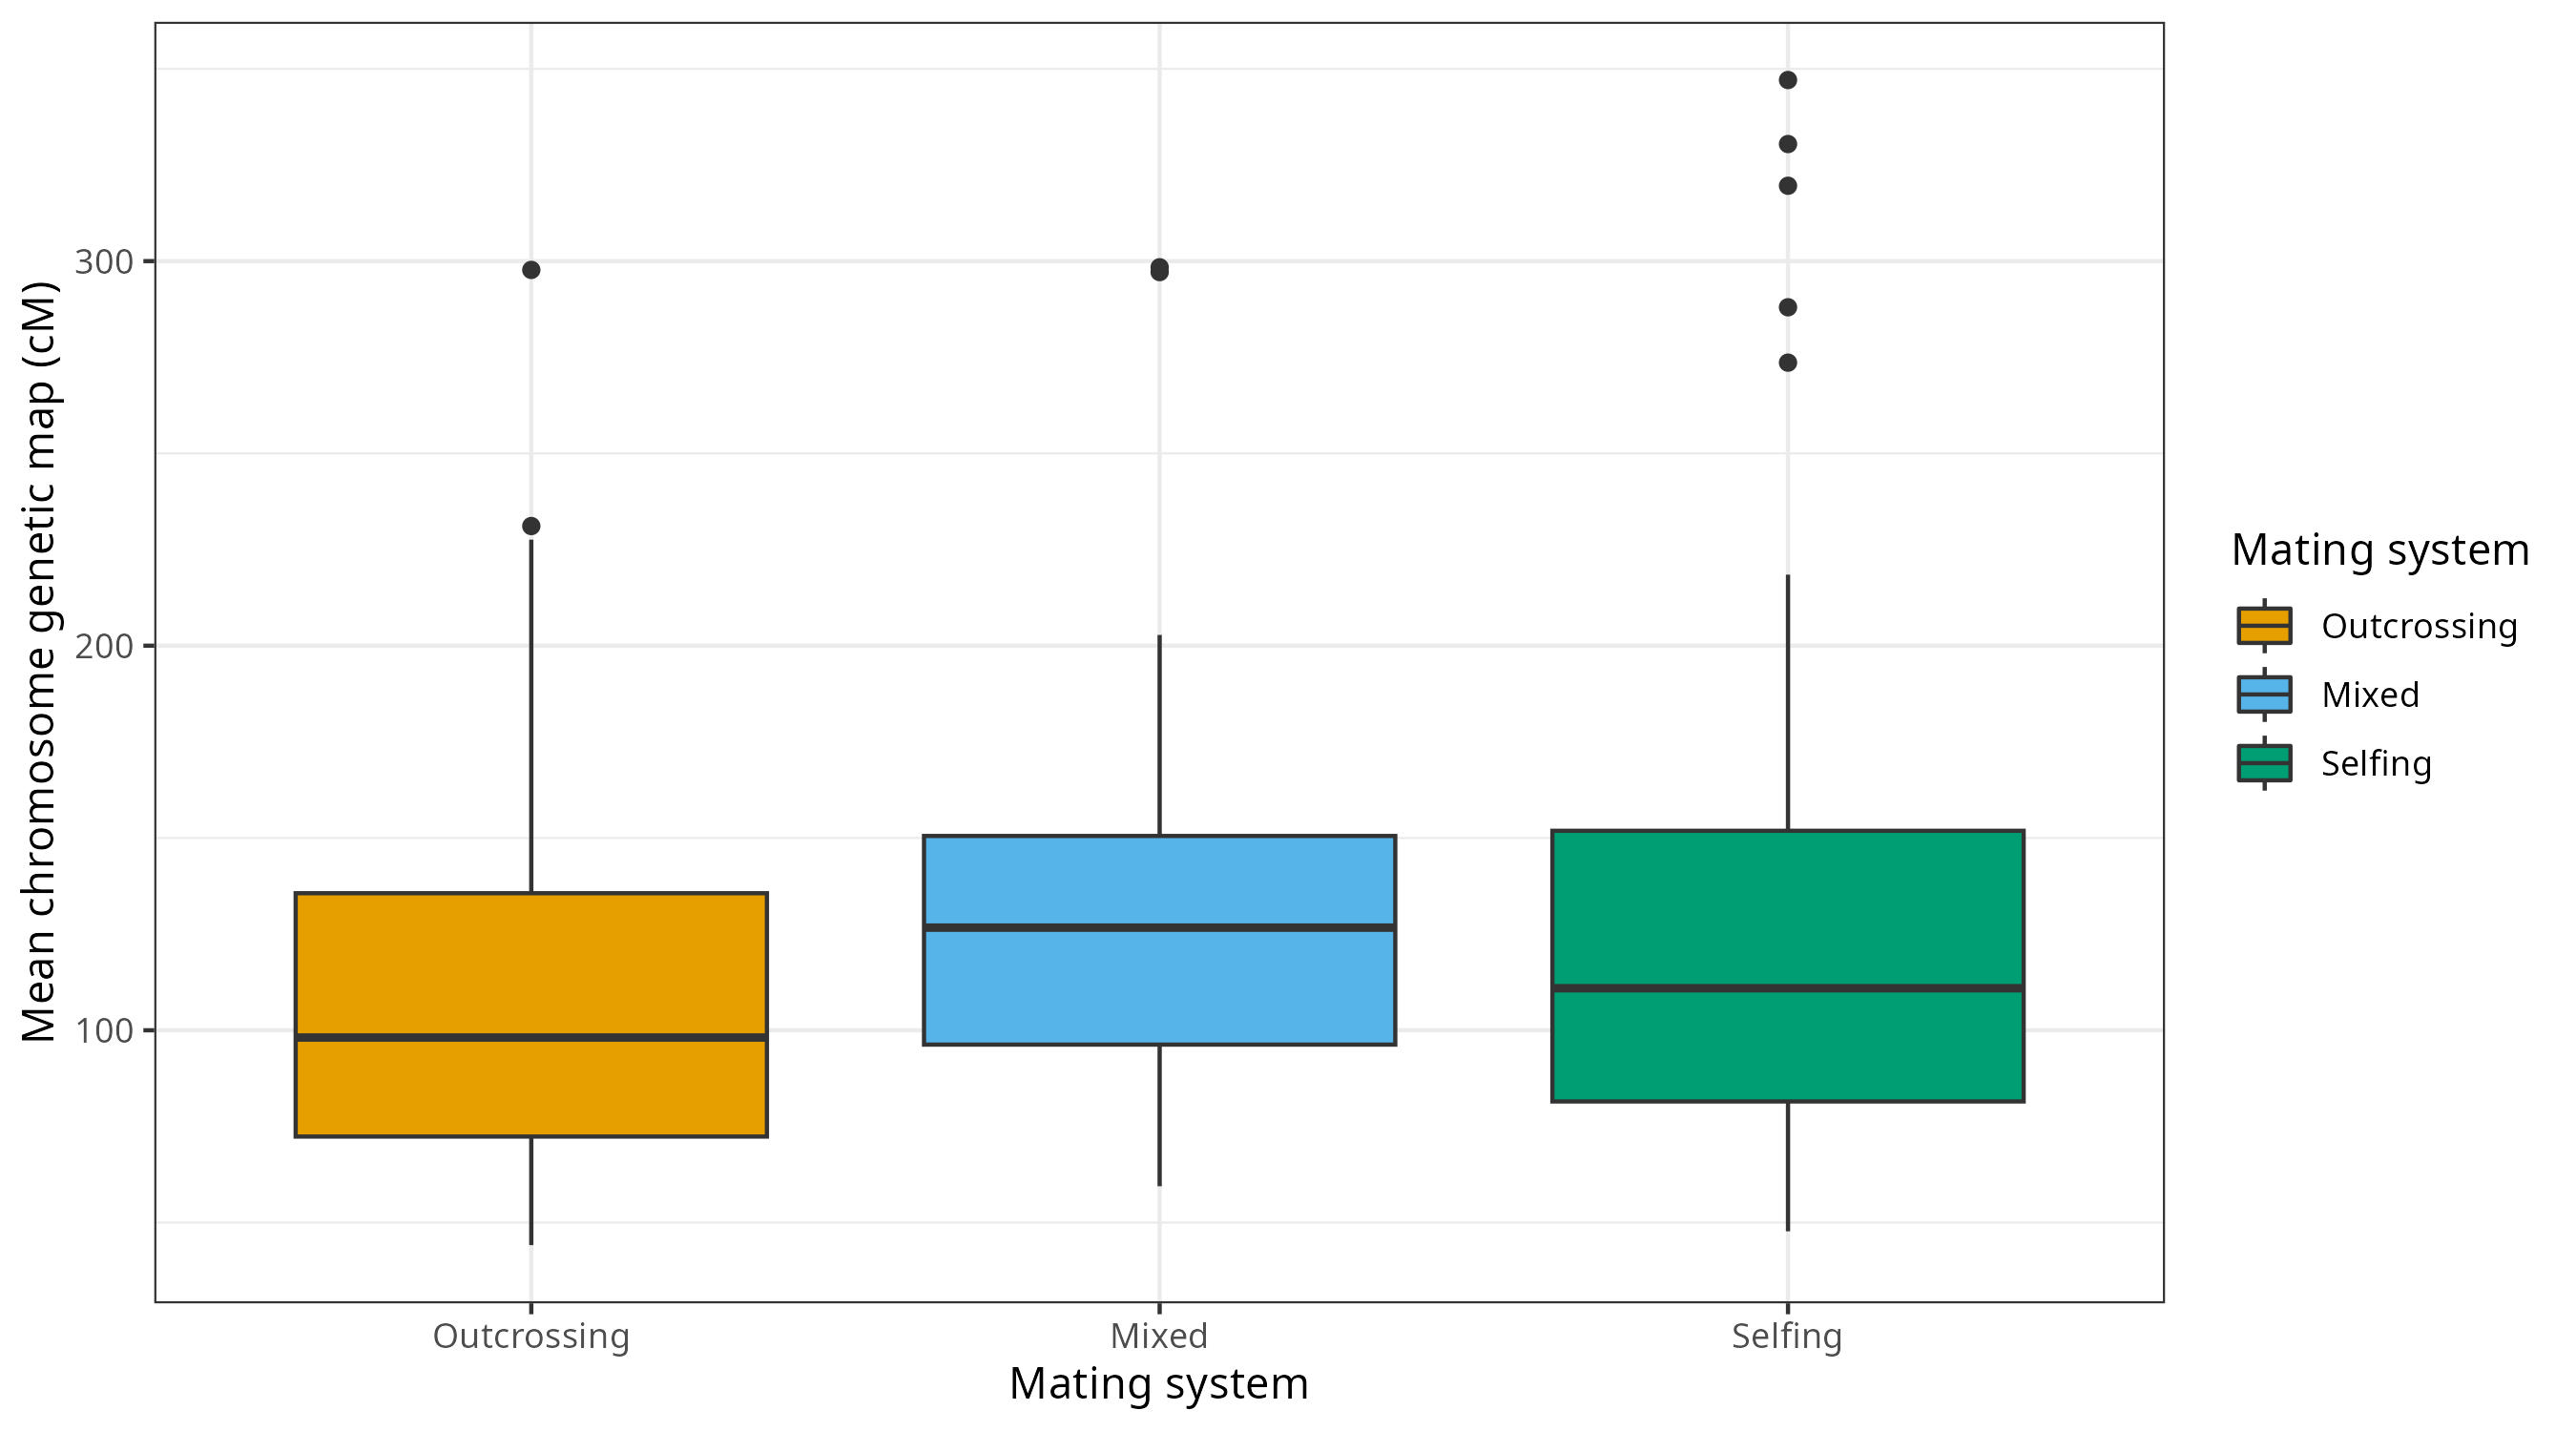
\includegraphics[width=0.9\textwidth]{figures/FigS3.jpeg}
  \centering
  \caption{Chromosome map length as a function of the mating system.
  }
  \label{figure:FigS3}
\end{figure}


\begin{figure}[h!]
  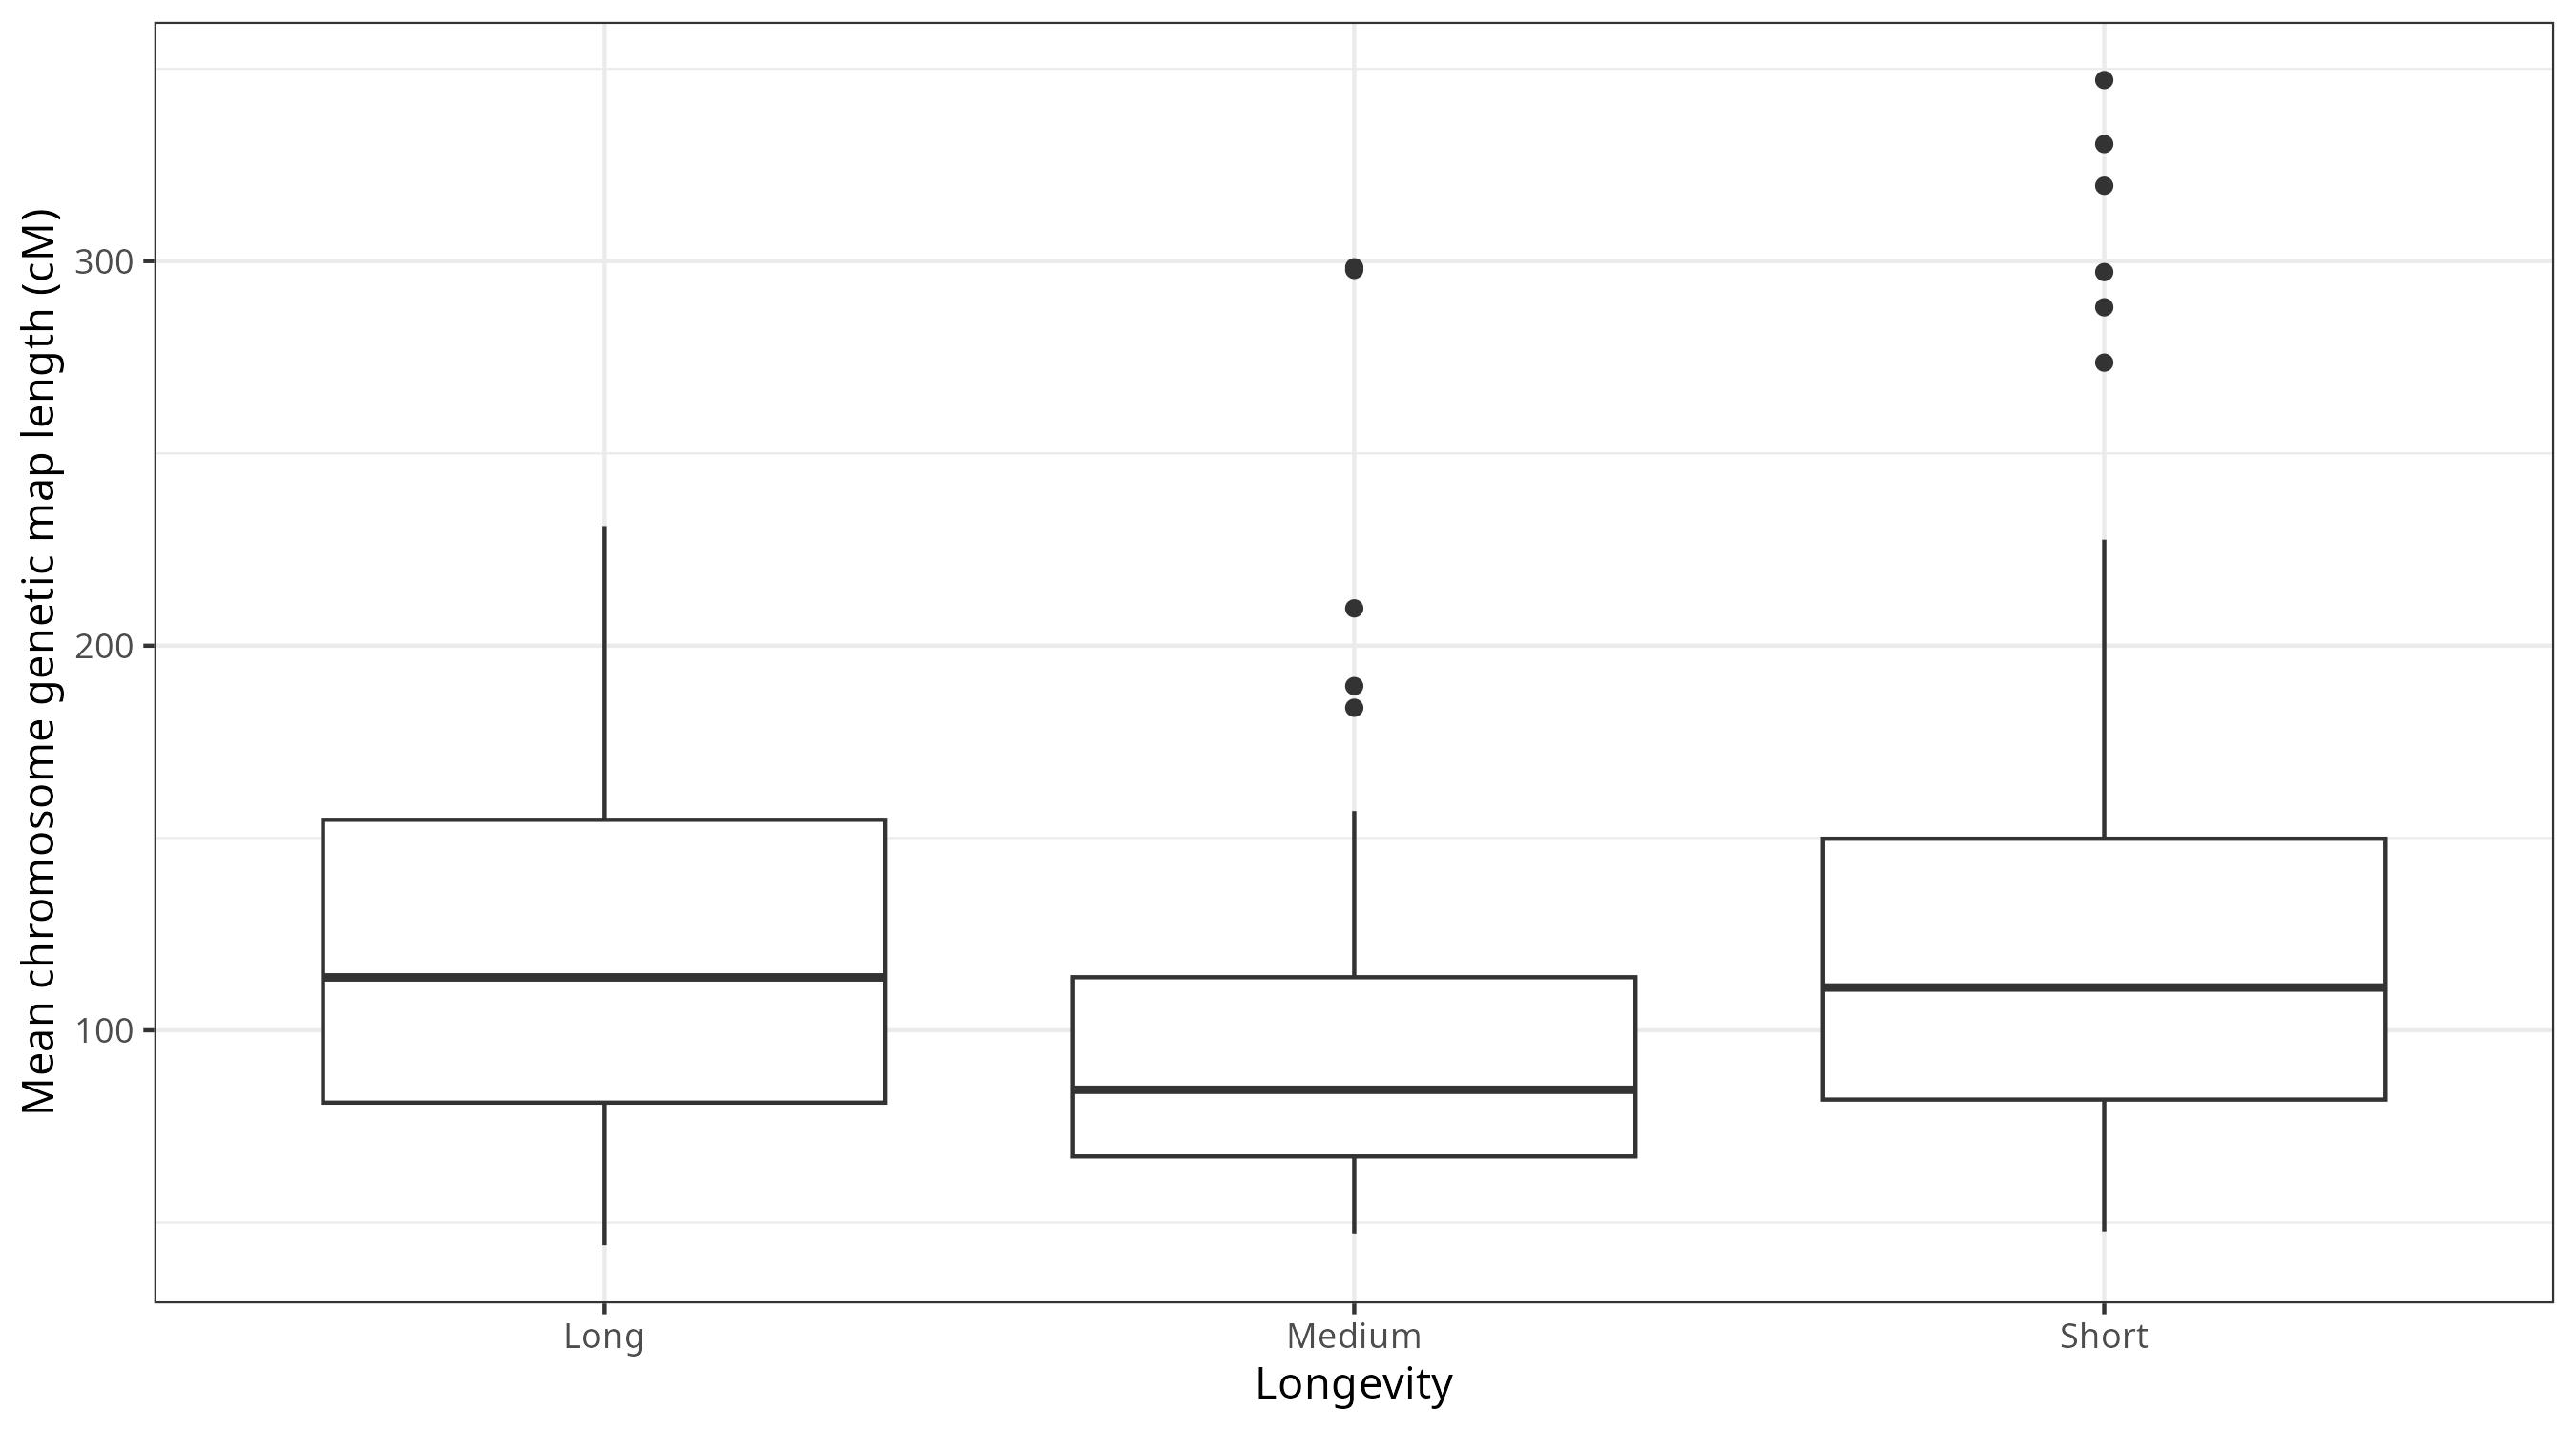
\includegraphics[width=0.9\textwidth]{figures/FigS4.jpeg}
  \centering
  \caption{Chromosome map length as a function of longevity.
  }
  \label{figure:FigS4}
\end{figure}


\begin{figure}[h!]
  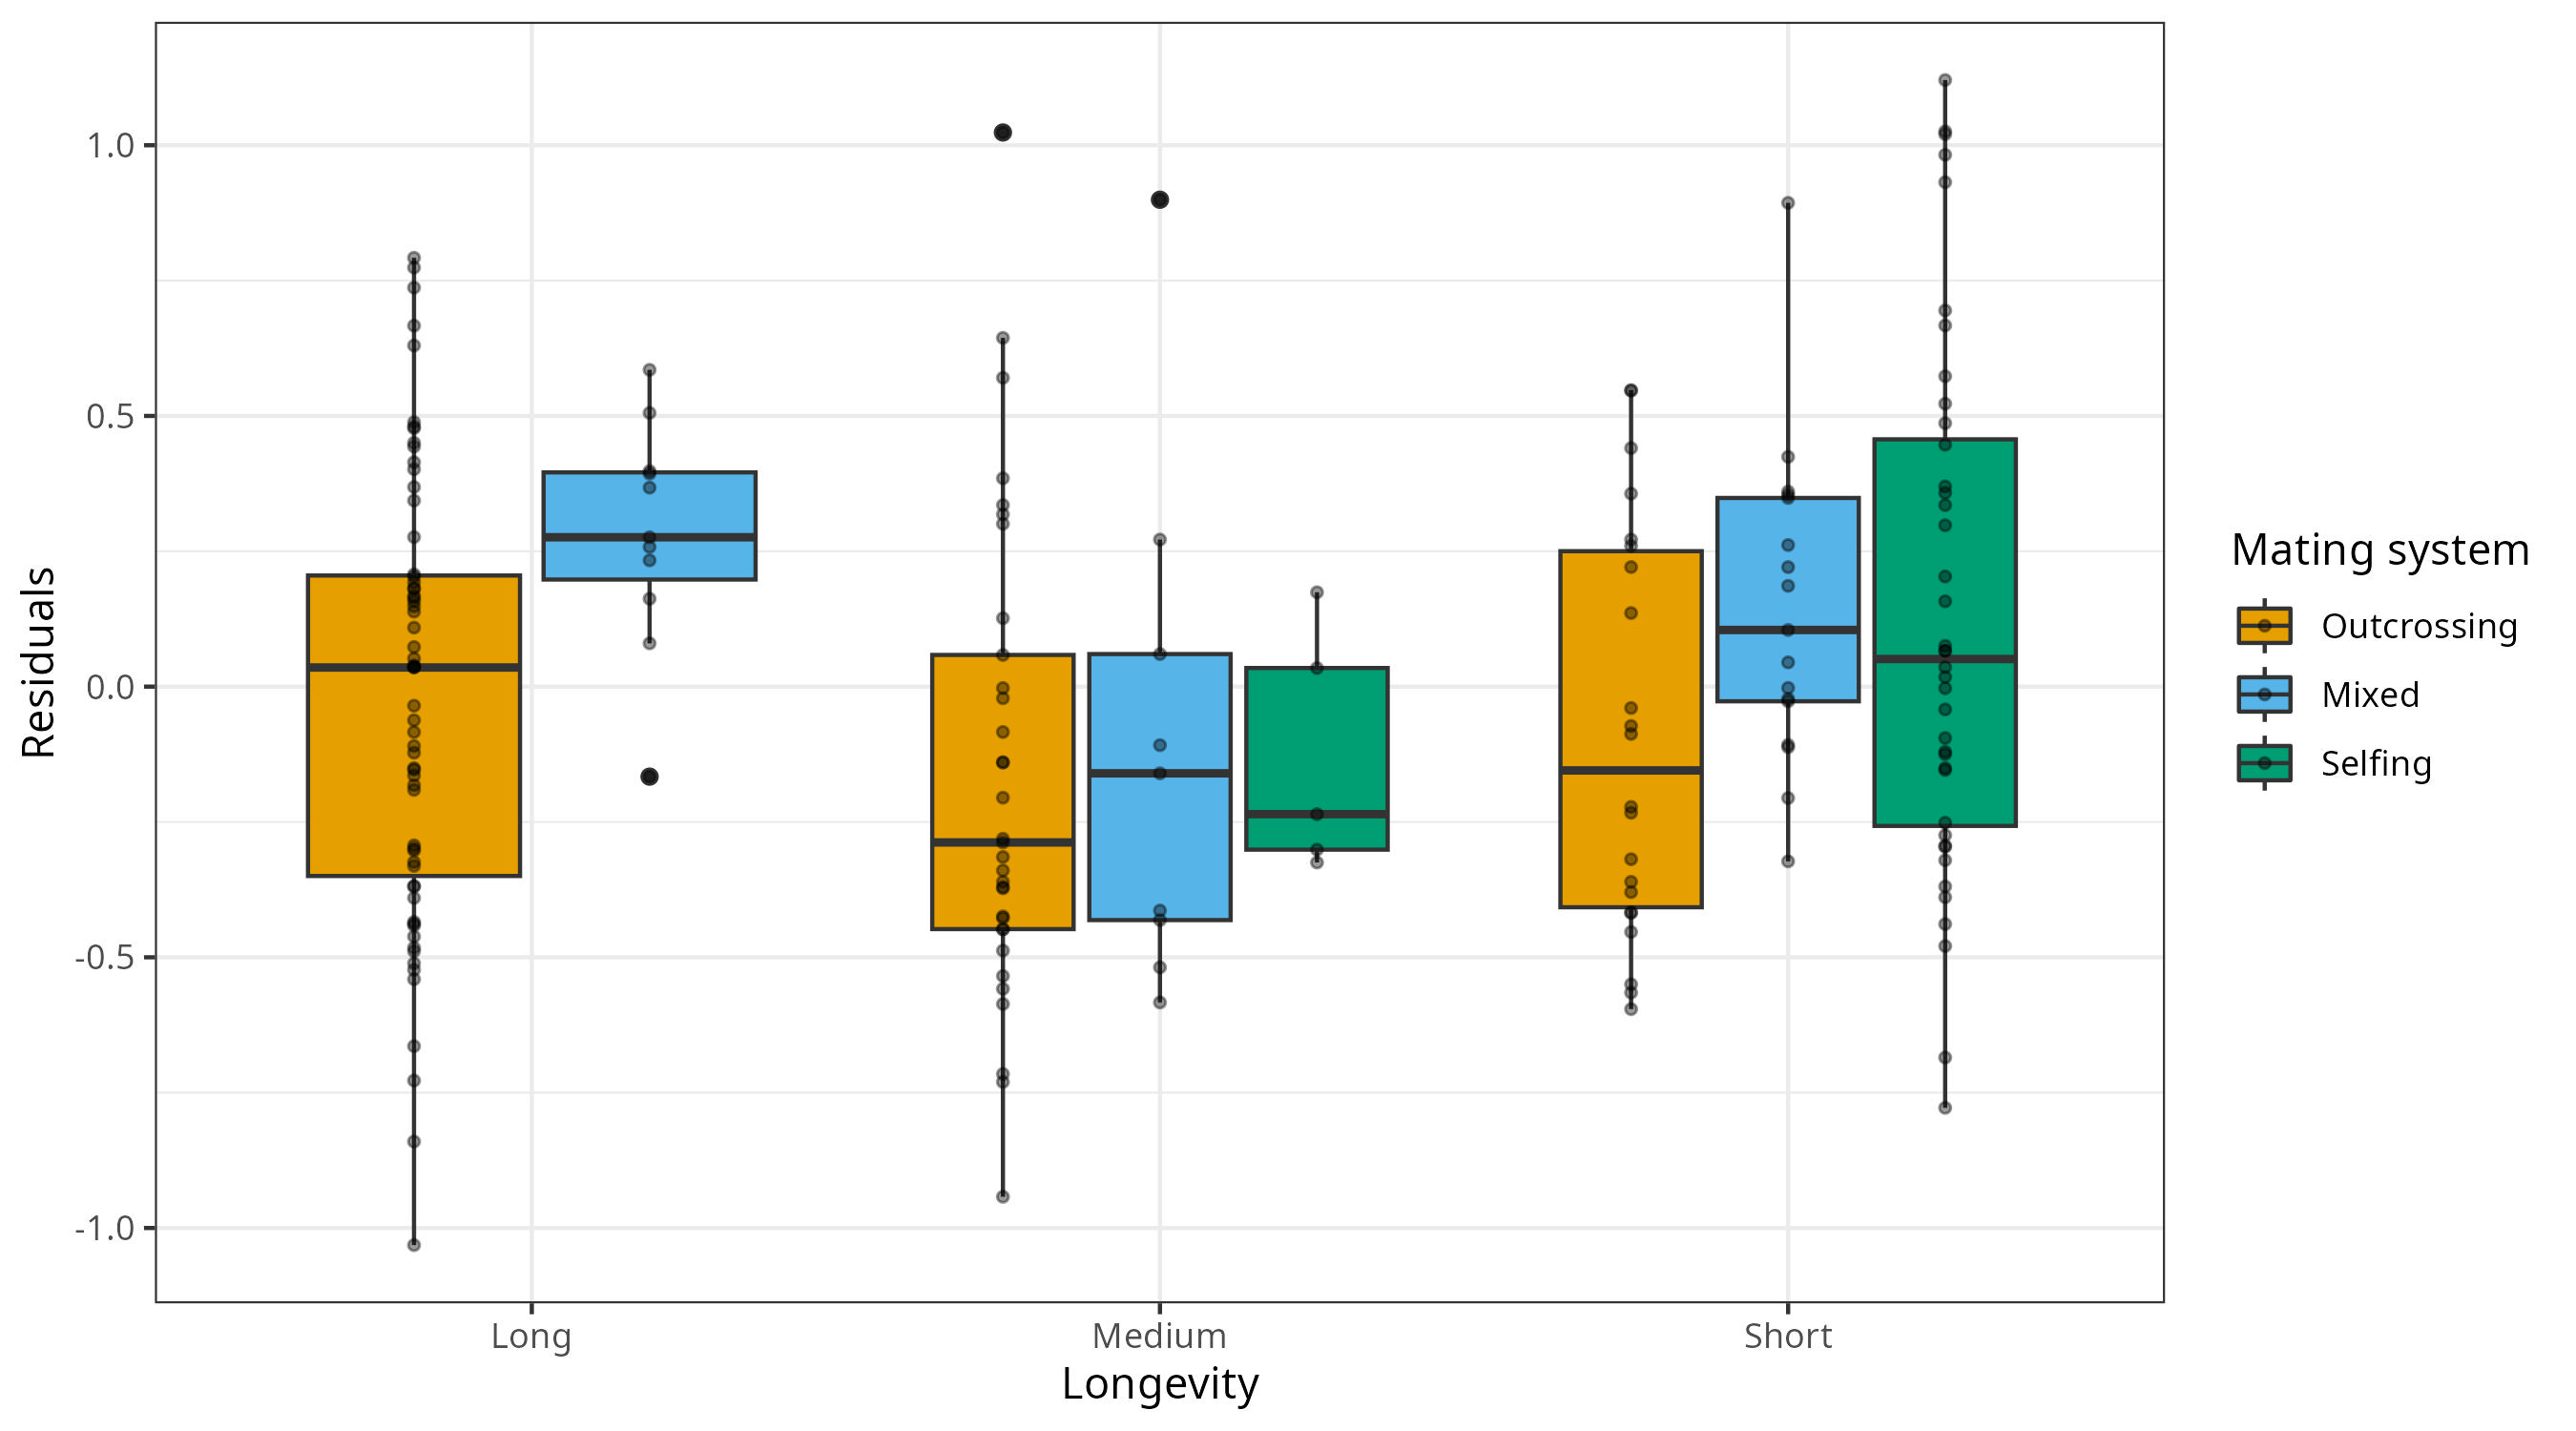
\includegraphics[width=0.9\textwidth]{figures/FigS5.jpeg}
  \centering
  \caption{The recombination rates depend on the mating system and longevity. The combined effect of the mating system and longevity on the residuals of the regression recombination rate (cM/Mb) ~ chromosome size(Mb).
  }
  \label{figure:FigS5}
\end{figure}




\clearpage

\section*{Supplementary tables}

\renewcommand{\thetable}{S\arabic{table}}

\setcounter{table}{0}


\begin{table}[h!]
\centering{}
\caption{Complete dataset with genetic map length, genome size, genomic characteristics (e.g. ploidy, number of chromosomes) and life history traits, associated with references.}
\begin{tabular}{cccccccc}
\end{tabular}
\label{table:tableS1}
\end{table}


\begin{table}[h!]
\centering{}
\caption{Forward model selection steps for the chromosome genetic map length and the residuals of the regression recombination rate ~ chromosome size. The Anova p-value and AIC/BIC values are provided for each 'lm' and 'pgls' model.}
\begin{tabular}{cccccccc}
\end{tabular}
\label{table:tableS2}
\end{table}



\begin{table}[h!]
\centering{}
\caption{Model fit and parameters estimates for the 'pgls' model testing the effect of the mating system, chromosome size, the interaction of the mating system and chromosome size, and the number of chromosomes. Chromosome genetic map length ~ mating system*chromosome size + chromosome number.}
\begin{tabular}{cccccccc}
\end{tabular}
\label{table:tableS3}
\end{table}


\begin{table}[h!]
\centering{}
\caption{Model fit and parameters estimates for the 'pgls' model testing the effect of marker density and number of progeny. Chromosome genetic map length ~ mating system + longevity + marker density + number of progeny.}
\begin{tabular}{cccccccc}
\end{tabular}
\label{table:tableS4}
\end{table}



\end{document}
